\documentclass{article}
%\documentclass[12pt,twoside]{report}
\usepackage[utf8]{inputenc}
%\usepackage{amsmath}
%\usepackage{amsfonts}
%\usepackage{amssymb}
\usepackage{float}
\usepackage{caption}
\usepackage{subcaption}
\usepackage{graphicx}
\graphicspath{ {Images/} }
\usepackage{xcolor}
\usepackage{listings}
\usepackage{multirow}
\usepackage[bottom=0.5in,margin=1in,footskip=0.4in, headsep=.2in]{geometry}
\usepackage{longtable}
%\usepackage{hyperref}
\usepackage{sectsty}
\usepackage{url}
\usepackage{array}
\usepackage{xcolor,colortbl}% http://ctan.org/pkg/xcolor
\usepackage{amssymb}
\usepackage{appendix}
%\usepackage{geometry}
%\usepackage[T1]{fontenc}
\newcommand{\done}{\cellcolor{green}}  %{0.9}
\newcommand{\hcya}[1]{{\cellcolor{yellow} #1}}
\newcommand{\hcy}[1]{{\cellcolor{orange} #1}}
\newcommand{\hcyan}[1]{{\cellcolor{red} #1}}
\newcommand{\hc}[1]{{\cellcolor{blue} #1}}

\newcommand{\package}[1]{ \texttt{ \textbf{#1}}}

\newcommand{\server}[1]{ \textit{#1}}


\newcommand{\file}[1]{  \texttt{ \textit{#1}}}
\newcommand{\unit}[1]{ \textrm{#1}}
\newcommand{\constant}[1]{ \textrm{\textit{#1}}}
\newcommand{\component}[1]{  \texttt{#1}}
\newcommand{\sensor}[1]{  \textit{#1}}
\newcommand{\option}[1]{  \texttt{#1}}
%\newcommand{\output}[1]{  \texttt{#1}}

%\lstdefinestyle{DOS}
%{
%	backgroundcolor=\color{white},
%	basicstyle=\scriptsize\color{black}\ttfamily,
%	xleftmargin=\parindent
%	
%%	basicstyle=\ttfamily,
%%	keywordstyle=\bfseries,
%%	showstringspaces=false,
%%	morekeywords={include, printf}
%
\lstset{
	basicstyle=\small\ttfamily,
	columns=flexible,
	breaklines=true
}

%
%\makeatletter
%\def\@@acrodef{\@ifstar\@acrodefs\@acrodef}
%\newtoks\acro@list
%\newcommand{\@acrodef}[2]{%
%	\global\acro@list=\expandafter{\the\acro@list\@elt{#1}{#2}}%
%	\global\@namedef{acro@#1}{n{#1}{#2}}}
%\newtoks\acro@resetlist
%\newcommand{\@acrodefs}[2]{%
%	\global\acro@resetlist=\expandafter{\the\acro@resetlist\@elt{#1}}%
%	\@acrodef{#1}{#2}}
%\def\acro@doresetlist{\begingroup
%	\def\@elt##1{\expandafter\expandafter\expandafter
%		\acro@reset\csname acro@##1\endcsname}\the\acro@resetlist\endgroup}
%\def\acro@reset#1#2#3{\global\@namedef{acro@#2}{n{#2}{#3}}}
%\newcommand{\acro}[1]{\expandafter\expandafter\expandafter
%	\use@acro\csname acro@#1\endcsname}
%\def\use@acro#1#2#3{\ifx n#1
%	#3 (#2)\global\@namedef{acro@#2}{o{#2}{#3}}%
%	\else
%	#2%
%	\fi}
%\newcommand{\listofacronyms}[1][tabular]{%
%	\begingroup\def\@elt##1##2{##1&##2\\}%
%	\@ifundefined{chapter}{\section*}{\chapter*}{\listacronymname}
%	\noindent\begin{#1}{@{}p{6em}p{\dimexpr\columnwidth-2\tabcolsep-6em\relax}@{}}
%		\the\acro@list
%	\end{#1}\endgroup}
%\providecommand\listacronymname{List of acronyms}
%\newenvironment{acronyms}{\let\acrodef\@@acrodef}{}
%\newenvironment{acronyms*}{\let\acrodef\@@acrodef}{\listofacronyms}
%\def\g@preto@macro#1#2{\toks0=\expandafter{#1}%
%	\toks2={#2}\xdef#1{\the\toks2 \the\toks0 }}
%\@ifundefined{chapter}
%{\g@preto@macro\section\acro@doresetlist}
%{\g@preto@macro\chapter\acro@doresetlist}
%\makeatother

%\usepackage[a4paper,width=150mm,top=25mm,bottom=25mm]{geometry}


\usepackage{fancyhdr}
\pagestyle{fancy}
\usepackage{fvextra}

\fancyhead{}
\fancyhead[RO,R]{\scalebox{1}{\begin{tabular}[b]{|c|c|c|}
			\hline
			\multirow{2}{*}{\quad\quad\quad \quad Pointing error investigation}&Doc No: & SSA-00000-000	\\
			\cline{2-3}
			&Rev No: & A\\
			\hline
\end{tabular}}}
\lhead{
\includegraphics[width=3cm]{logo2.png}}

\fancyfoot{}
%\fancyfoot[L,RO]{\thepage}
\rfoot{Page \thepage \hspace{1pt} of \pageref{LastPage}}
%\fancyfoot[LO,CE]{Chapter \thechapter}
%\fancyfoot[CO,RE]{Author Name}
\lfoot{ \textbf{Form Number (To be Allocated) Rev 01}\\
	{\fontsize{6.5}{6.7} \selectfont This document is the property of SARAO and shall not be used, reproduced, transmitted or disclosed without prior written permission.}}

\renewcommand{\footrulewidth}{0.4pt}% default is 0pt
\renewcommand{\headrulewidth}{0pt}% default is 0pt
%\rfoot{footer}
 
%\usepackage{biblatex}
%\addbibresource{references.bib}

\newcolumntype{R}[1]{>{\raggedleft\let\newline\\\arraybackslash\hspace{0pt}}m{#1}}


%TEXT\parencite[see][p10]{latexcompanion}
%TEXT\parencite[compare][]{knuthwebsite}
%TEXT\parencite[e.g.][page 300]{einstein}


\title{
	{
\includegraphics[width=12.3cm]{logo2.png}}\\
	\vspace{1.5cm}
	\vspace{1.5cm}
	{MeerKat Dish Pointing Error Investigation : \\ Wind and Temperature Factors }\\
	{\large SARAO}\\
	\vspace{1.5cm}
}
\vspace{1.5cm}
\vspace{1.5cm}
\author{Authors: Moloko Hlakola}
\date{}
\begin{document}
\maketitle
\clearpage

\section*{}

\begin{table}[h]
		\textbf{\centerline{DOCUMENT APPROVALS}}

	\begin{tabular}[b]{|c|c|c|c|c|c|}
	\hline
	&	\textbf{Name}&	\textbf{	Designation}&		\textbf{Affiliation}&	\textbf{	Date}&		\textbf{Signature}\\
	\hline
	\textbf{Prepared By}&M Hlakola&	Operator&	SARAO&	&\\	
	\hline
	\textbf{Reviewed By}&	Ops Team&	Operators&	SARAO&	&	N/A\\
	\hline
	\textbf{Accepted By}&	C Gumede&	Telescope Operations& Manager&	&SARAO\\
	\hline
	\textbf{Approved By}&	L Magnus&	Head: Operations&	SARAO&&\\
	
	\hline
\end{tabular}	
\end{table}

\begin{table}[h]
	\textbf{\centerline{DOCUMENT HISTORY}} 

\begin{tabular}[b]{|c|c|c|c|}
	\hline
	{\fontsize{8}{3}\selectfont \textbf{Revision}}&{\fontsize{8}{3}\selectfont						\textbf{Date Of Issue}}&	\textbf{Prepared By}&	{\fontsize{8}{3}\selectfont	\textbf{Comments (e.g. ECN Number or changes to document)}}\\
	\hline			
{\fontsize{10}{4}\selectfont	A}	&{\fontsize{10}{4}\selectfont								12-04-2021}&	{\fontsize{10}{4}\selectfont M Hlakola}&{\fontsize{10}{4}\selectfont	Issued for Comments} \& {\fontsize{10}{4}\selectfont Review}\\ 
	
	\hline
\end{tabular}
\end{table}
\begin{table}[h]


\textbf{\centerline{DOCUMENT DISTRIBUTION}} 
\begin{tabular}[b]{|p{15.5cm}|}
	\hline
	{\fontsize{10}{4}\selectfont This the initial draft of the document. The has been submitted for review}\\
	\hline
\end{tabular}
\end{table}

\begin{table}[H]

\textbf{\centerline{DOCUMENT SOFTWARE}} 

%\centering
\resizebox{\textwidth}{!}{%
	\begin{tabular}[b]{|p{2cm}|p{2cm}|p{2cm}|p{7.4cm}|}
	
	\hline
	
	\multicolumn{2}{|c|}{\textbf{Package}}	& \textbf{Version}	& \textbf{Filename}\\
	\hline
	Latex&TexStudio & 	N/A& Meerkat\_Settings \\
	\hline
\end{tabular}

}
\end{table}

\textbf{\centerline{COMPANY DETAILS}} 
\resizebox{\textwidth}{!}{%
	\begin{tabular}[b]{|p{3cm}|p{4.1cm}|p{4.1cm}|p{4.1cm}|p{4.1cm}|}
		\hline
		
		Name & 
		SKA SA, Johannesburg Office
		(Rosebank, Gauteng)
		
		& 
		SKA SA, Cape Town Office
		(Pinelands, Western Cape)
		
		& 
		SARAO, HartRAO
		(Hartebeeshoek, Gauteng)&SARAO, Karoo Astronomy Reserve
		(Carnarvon, Northern Cape)   \\
		
		\hline
		
		Physical/Postal
		Address
		
		&
		1$^{st}$ Floor, 17 Baker Street 
		Rosebank, Gauteng
		2196, South Africa
		&
		
		3rd Floor, The Park,
		Park Road, Pinelands,
		7405, South Africa
		
		& 
		P.O.Box 443, Krugersdorp 1740, South Africa 
		
		&
		Posbus 69, Carnarvon, 8925, South Africa\\
		
		\hline
		
		
		Tel.&
		+27 11 268 3400&
		+27 21 506 7300&
		+27 (12) 301-3100&
		+27 21 506 7300\\
		
		\hline
		
		Fax.&
		27 11 442 2454&
		+27 21 506 7375&
		+27 (12) 301-3300&
		+27 (0)86 538 6836\\
		
		\hline
		Website&
		www.ska.ac.za&
		www.ska.ac.za&
		www.hartrao.ac.za&
		www.ska.ac.za\\
		\hline	
		
	\end{tabular}
	|}
\clearpage




	\section*{}
{
\includegraphics[width=16cm]{logo2.png}}
\vspace{1cm}
\vspace{1cm}

{\color{red}\textbf{\centerline{MeerKat Dish Pointing Error Investigation : Wind and Temperature Factors}} }

{\color{red}\begin{tabular}[b]{p{8cm} R{7.6cm}}

	

	Document number&	SSA-00000-00\\
	Revision&	A\\
	Classification&	Commercial in Confidence\\
	Prepared By	& M Hlakola\\                              
	Approval Date &	01 02 2021\\
	

\end{tabular}
}
\vspace{1cm}
\vspace{1cm}
\vspace{1cm}

{\color{red}\begin{tabular}[b]{p{6cm}p{0.2cm}p{9cm}}
	
	\hline	
	
	Organisation&	:&
	NRF (National Research Foundation)\\
	Facility	&:&
	SARAO (South African Radio Astronomy Observatory)\\
	Project	&:&
	N/A\\
	Document Type	&:&
	Guidelines (UG)\\
	Function/Discipline&	:&
	Operations Management (0006)\\
	\hline
\end{tabular}
}
\clearpage

 \listoffigures
%\addcontentsline{toc}{section}{List of Figures}
%  \listoffigures\newpage.
% 

% \addtocontents{toc}{\protect\contentsline{chapter}{\listfigurename}{\getpagerefnumber{listoffigures}}}
% \addtocontents{toc}{\protect\contentsline{chapter}{\listtablename}{\getpagerefnumber{listoftables}}}


\listoftables 
%\addcontentsline{toc}{section}{List of Tables} 
\tableofcontents

\section{Introduction}
In this study we investigate causes of drifts in Interferometric Pointing model parameters of the Meerkat Radio Telescope. The telescope comprises 64 13-m off-set gregorian dishes[\cite{Tony}].  A detailed description of the model is  provided in [\cite{Tony}]. In general, pointing errors are caused by poor modeling atmospheric refraction, manufacturing and assembling errors, structural deformations caused by gravity, wind and temperature.[\cite{Bayley}].  Antenna structure tilts caused by differential heating from solar illumination (depending on the weather up to
about 50 arcseconds) and wind[\cite{Tony}] is still under investigation. Therefore, the study focuses on the effects of temperature (differential heating from solar illumination) and wind on the pointing accuracy shift.  Data was collected from 01 Jan 2021 to 31 May 2021 to cover both extreme cold and hot weather conditions.  

\section{Approach}

The instrument is relatively new with a number of misunderstood assembly errors, components misalignment during preventative and corrective maintenance activities, and slipages during operations.  Therefore, pointing model issues which are caused by isolated instances of misfitted and faulty components are investigated separately and listed in \textbf{Appendix A and B}.   \\
\\
The Pointing Check script progress outputs (L-band) from 01 Jan 2021 to 31 May 2021 were downloaded and processed to extract data for m009 and m033 pointing shifts (See \textbf{Appendix C} for the python used to process data).  The script calculates the error of pointing (in arcmin) in terms of azimuth and elevation angles.  The error shows how much pointing accuracy has shifted over time in comparison to the existing pointing model derived from Interferometric Pointing[\cite{Tony}].  The time period covers summer and winter days for investigation of the weather factors.  Temperature, wind and tilt sensor data was collected from CAM GUI for the given time periods. \\

Collected data is plotted and analysed to identify patterns of pointing model drifts under different temperature and wind conditions.     


\section{Collection of Data}
The following figures show plots of azimuth and elevation shifts (error) extracted from Pointing Check progress outputs for m033 and m009 respectively.  The bash command in \textbf{Appendix C} was used to extract data from the progress output logs and a five column (\textit{date-time, azim, elev, azim-error, elev-errr}) csv file was downloaded as shown in \textbf{Figure}~\ref{fig:data2}.  Sensor data of average wind and temperature  was downloaded as csv file as shown in \textbf{Figure}~\ref{fig:temp2} and \textbf{Figure}~\ref{fig:wind3} 

\begin{figure}[H]
	%	\centering
	%\includegraphicsdpi{100}{}{bur1.png}     
	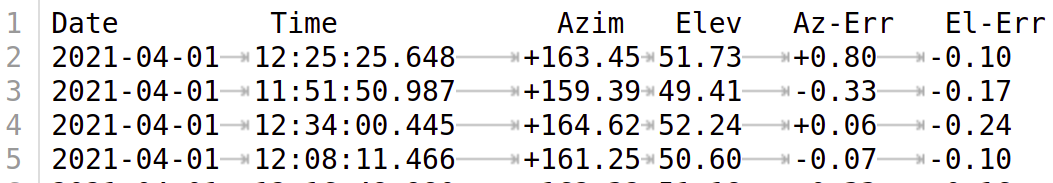
\includegraphics[scale=0.42]{data2.png}
	
	%\includegraphics[resolution=100]{bur1.png}
	\caption{Data extracted from the Pointing Script progress output (in csv format).}
	\label{fig:data2}
\end{figure}

\begin{figure}[H]
	%	\centering
	%\includegraphicsdpi{100}{}{bur1.png}     
	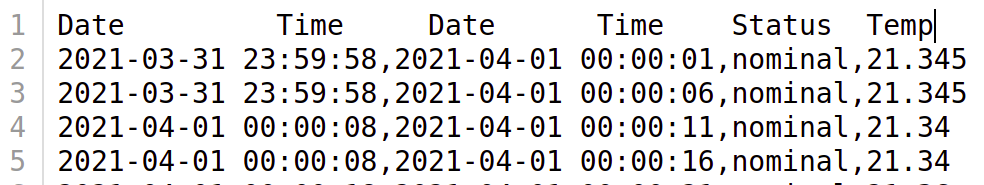
\includegraphics[scale=0.42]{temp2.png}
	
	%\includegraphics[resolution=100]{bur1.png}
	\caption{Enviromental air temperature data format (CSV file)}
	\label{fig:temp2}
\end{figure}
\begin{figure}[H]
	%	\centering
	%\includegraphicsdpi{100}{}{bur1.png}     
	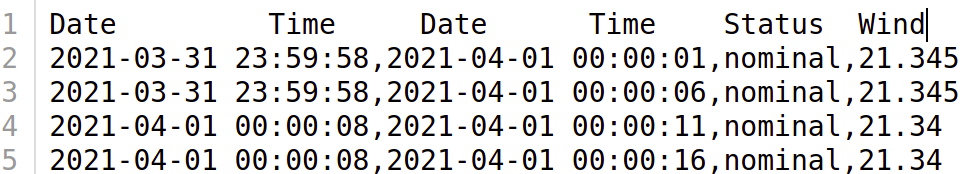
\includegraphics[scale=0.43]{wind3.png}
	
	%\includegraphics[resolution=100]{bur1.png}
	\caption{Enviromental wind speed data format (CSV file)}
	\label{fig:wind3}
\end{figure}

\subsection{Wind and Temperature Patterns  }
Screens shots of mean wind speed and air temperature plots from CAM GUI are shown in \textbf{Figure}~\ref{fig:wind1} and \textbf{Figure}~\ref{fig:temp1} repectively.  This is only sample data over the first 15 days of Jan 2021 for illustrution of weather patterns at the Meerkat Telescope site.

\begin{figure}[H]
	\centering
	%\includegraphicsdpi{100}{}{bur1.png}     
	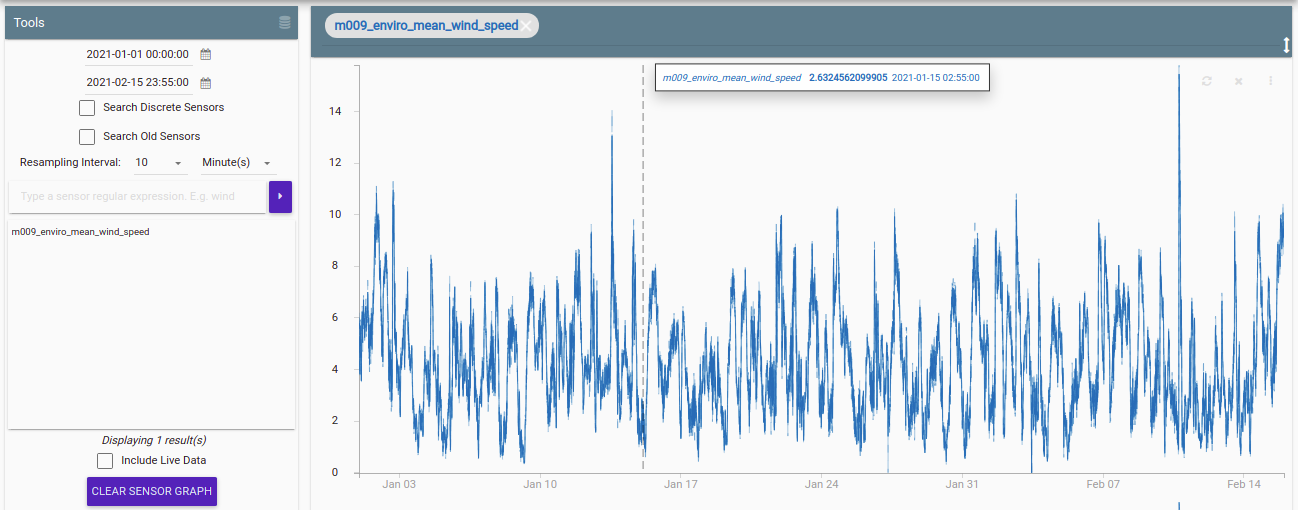
\includegraphics[scale=0.33]{m009_wind_Jan_partten.png}
	
	%\includegraphics[resolution=100]{bur1.png}
	\caption{Plot of everage wind speed  in Jan 2021}
	\label{fig:wind1}
\end{figure}
\begin{figure}[H]
	\centering
	%\includegraphicsdpi{100}{}{bur1.png}     
	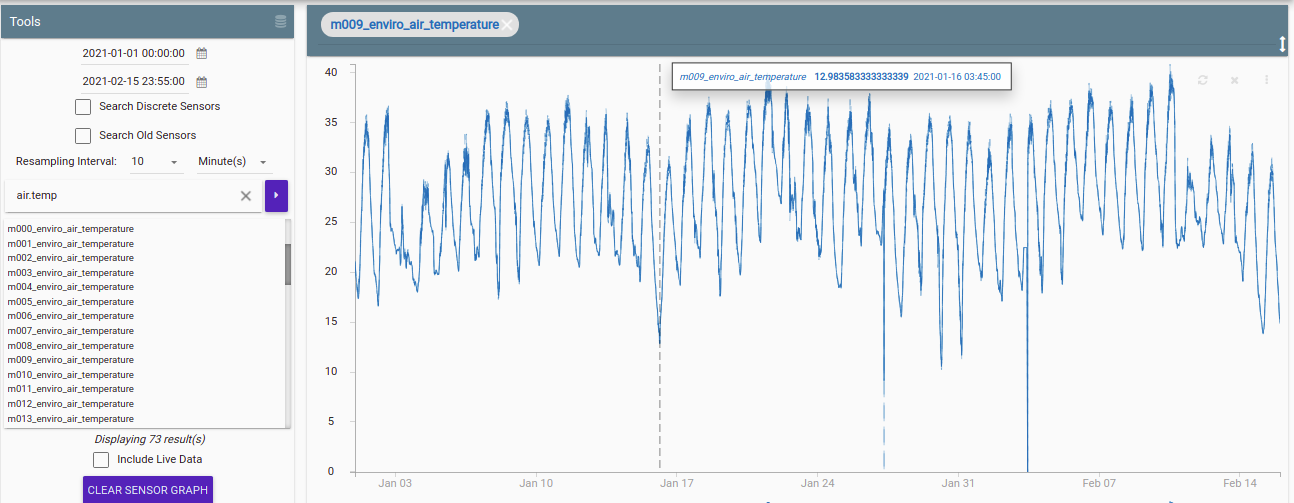
\includegraphics[scale=0.33]{m009_Jan_air_tep.png}
	
	%\includegraphics[resolution=100]{bur1.png}
	\caption{Plot of air temperature in Jan 2021}
	\label{fig:temp1}
\end{figure}



\subsection{Antenna m033 Pointing Check Script Data  }
Plots of m033 pointing errors (adjustments) in elevation and azimuth are shown in \textbf{Figure}~\ref{fig:m033ElevJan} to \textbf{Figure}~\ref{fig:m033AzimMay}.  The top left plots show pointing error elevation or azumuth againts time of the day.  The top right plot show the refracted azimuth or elevation angle with the error bar.   The bottom left and right show air temperature and wind speed for one day (01 Jan) respectively.




\begin{figure}[H]
	%	\centering
	%\includegraphicsdpi{100}{}{bur1.png}     
	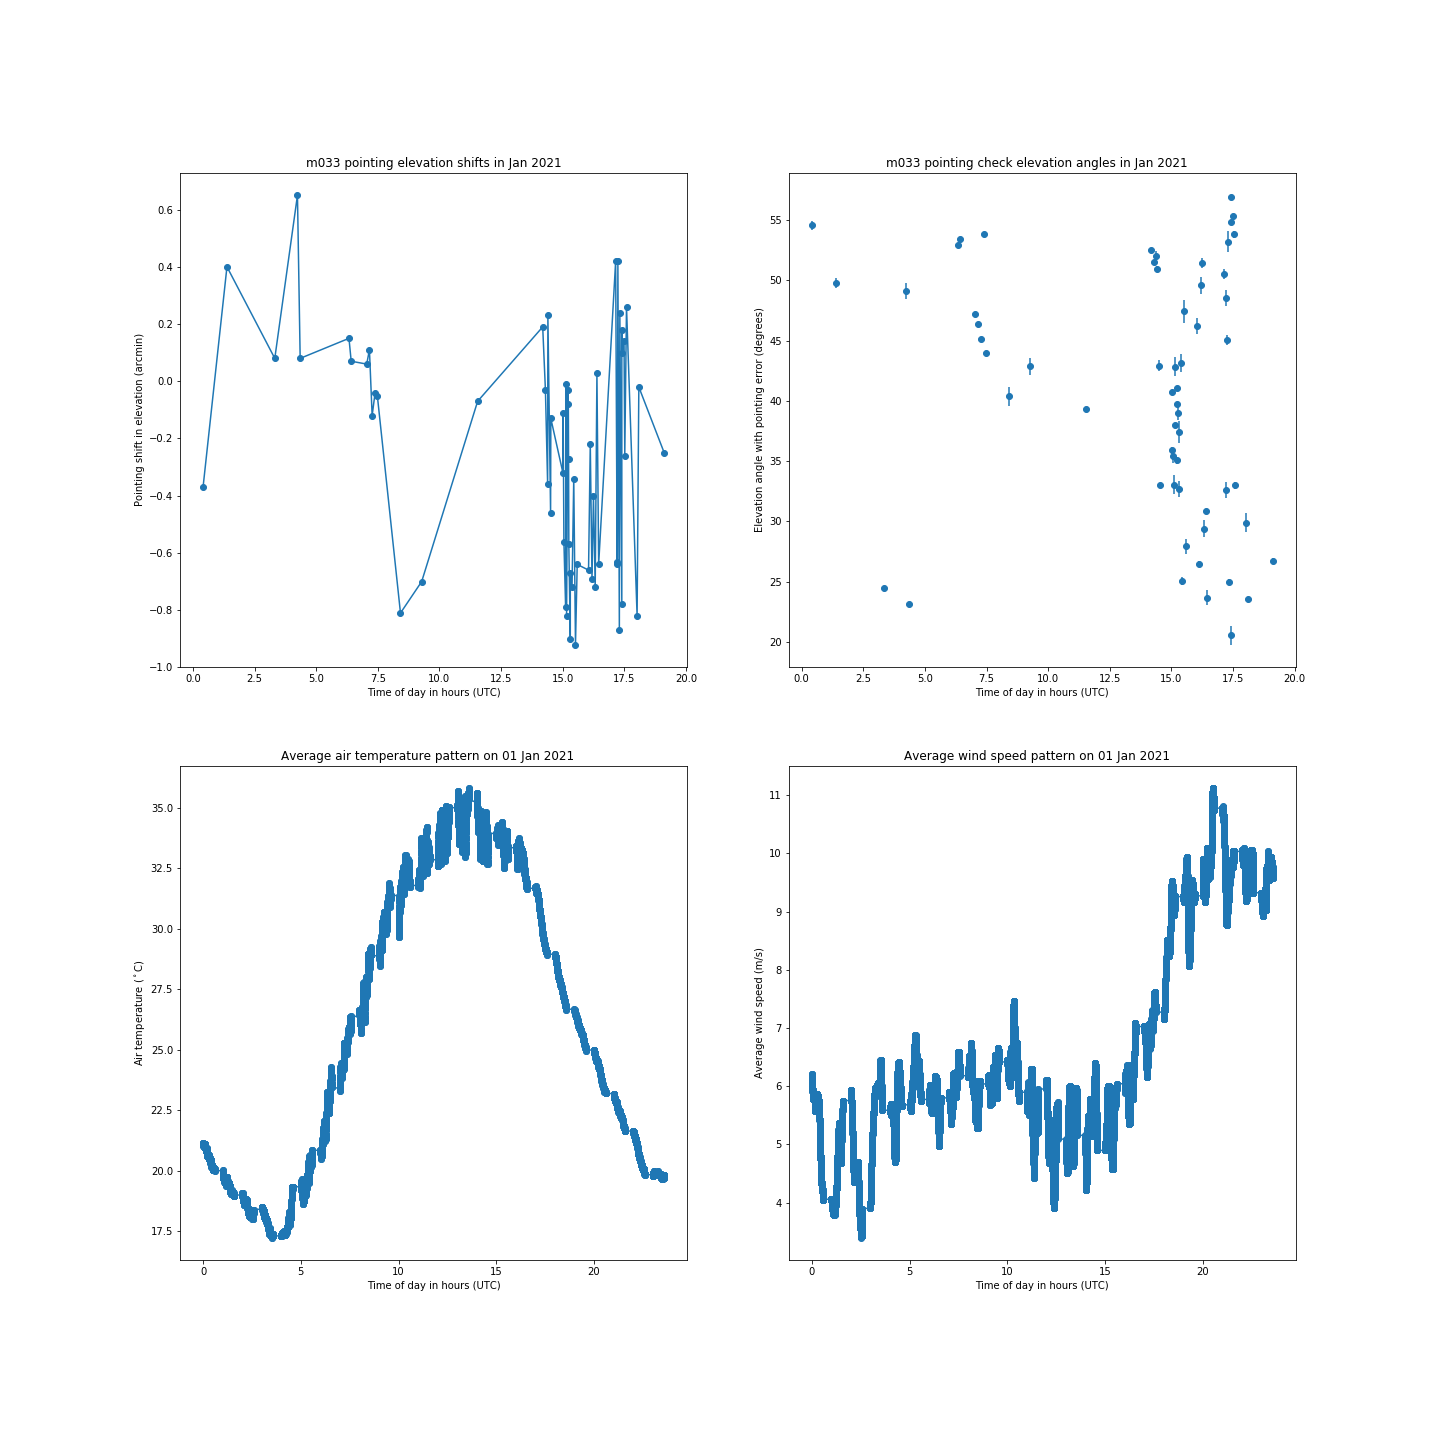
\includegraphics[scale=0.35]{m033_elev_Jan.png}
	
	%\includegraphics[resolution=100]{bur1.png}
	\caption{Plots of pointing error in elevation, angle of elevation, temperature and wind against time}
	\label{fig:m033ElevJan}
\end{figure}

\begin{figure}[H]
	\centering
	%\includegraphicsdpi{100}{}{bur1.png}     
	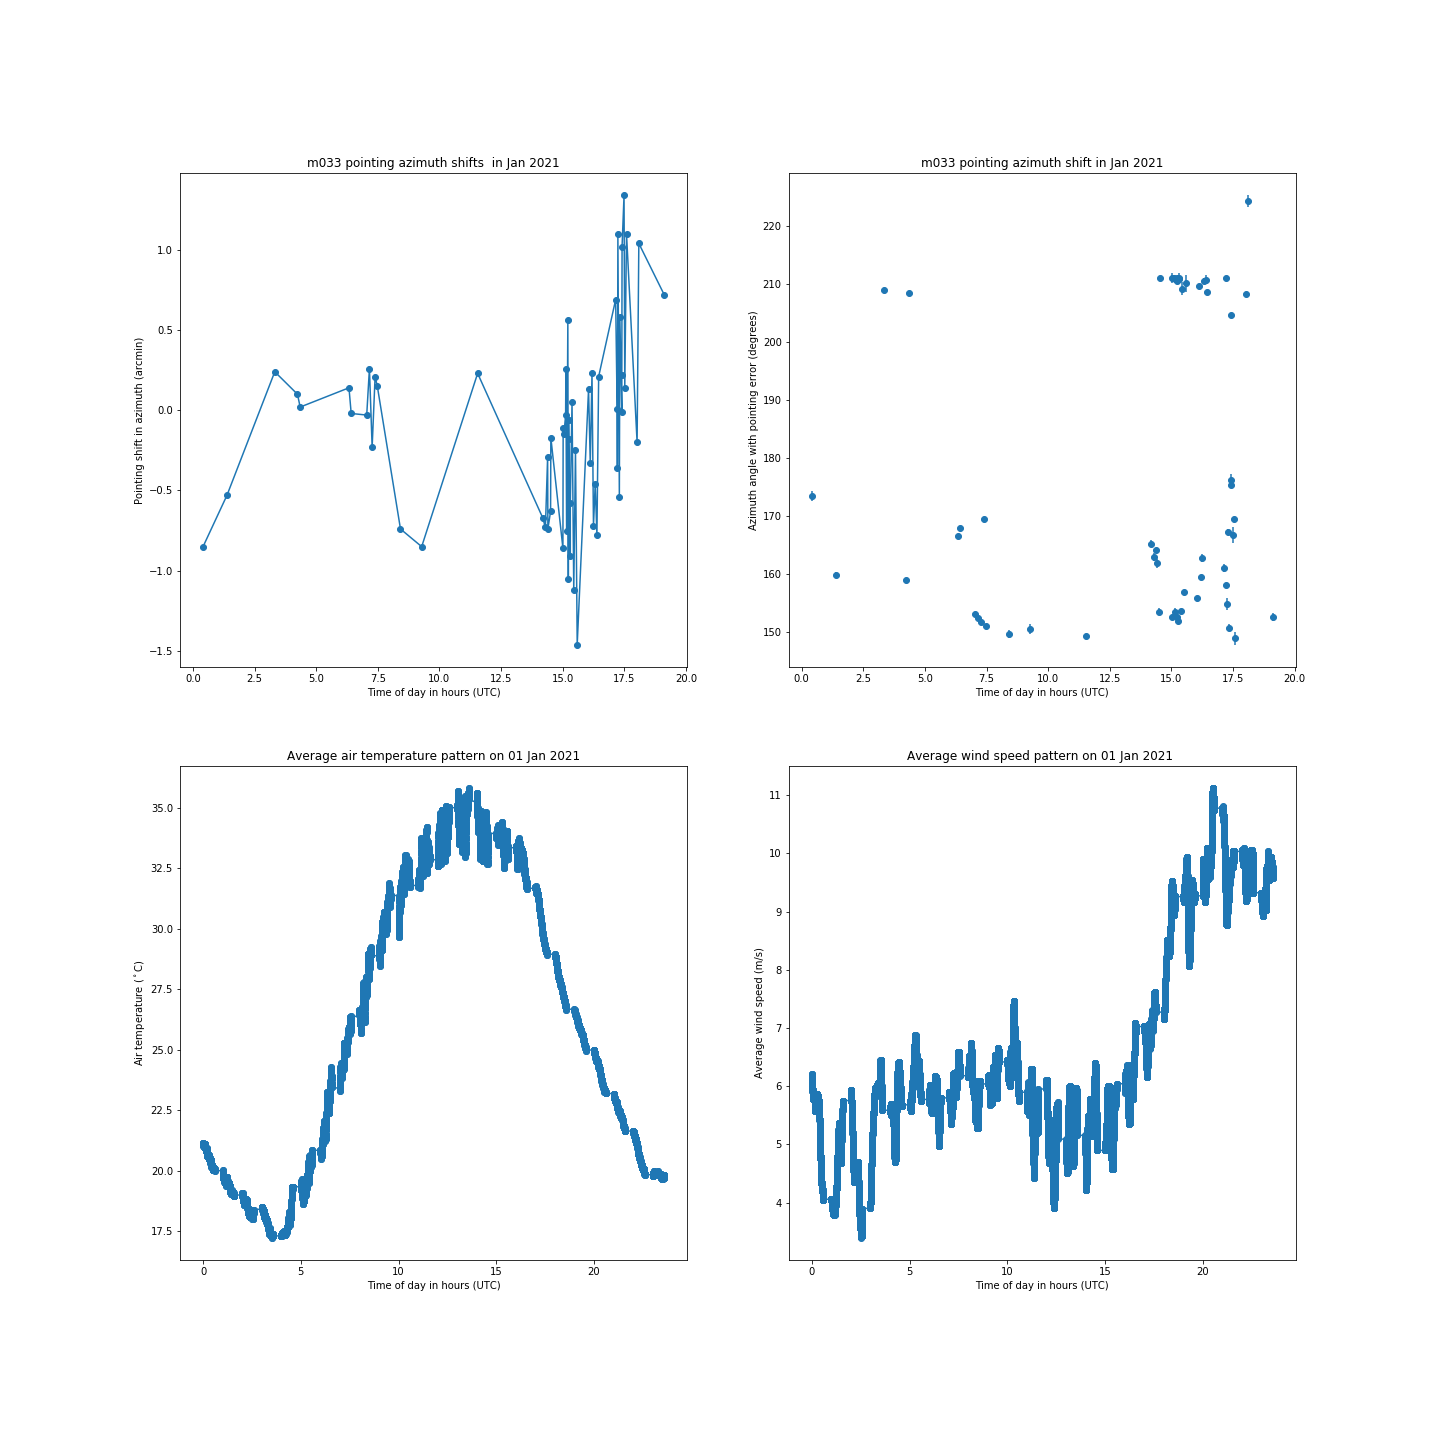
\includegraphics[scale=0.35]{m033_azim_Jan.png}
	
	%\includegraphics[resolution=100]{bur1.png}
	\caption{Plots of pointing error in azimuth, angle of azimuth, temperature and wind against time.}
	\label{fig:m033AzimJan}
\end{figure}

\begin{figure}[H]
	\centering
	%\includegraphicsdpi{100}{}{bur1.png}     
	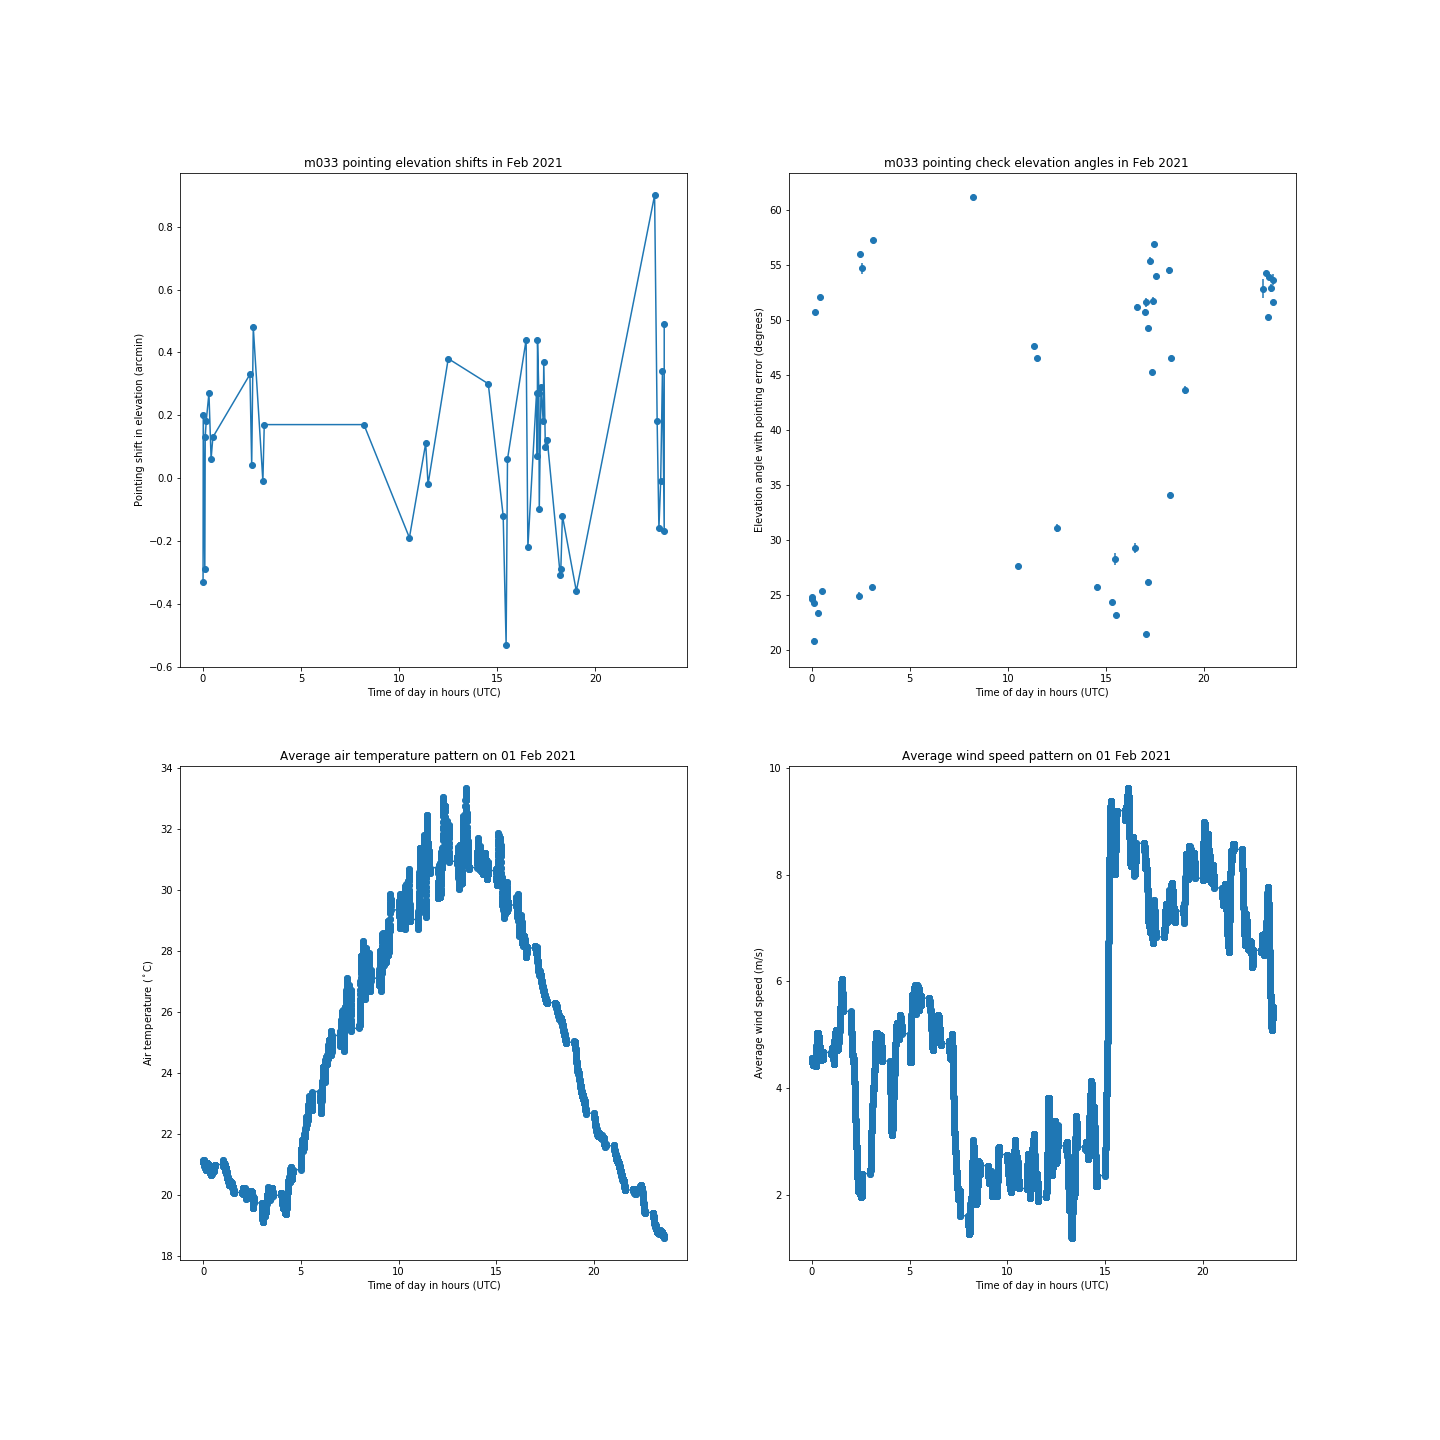
\includegraphics[scale=0.35]{m033_elev_Feb.png}
	
	%\includegraphics[resolution=100]{bur1.png}
	\caption{Plots of pointing error in elevation, angle of elevation, temperature and wind against time}
	\label{fig:m033ElevFeb}
\end{figure}

\begin{figure}[H]
	\centering
	%\includegraphicsdpi{100}{}{bur1.png}     
	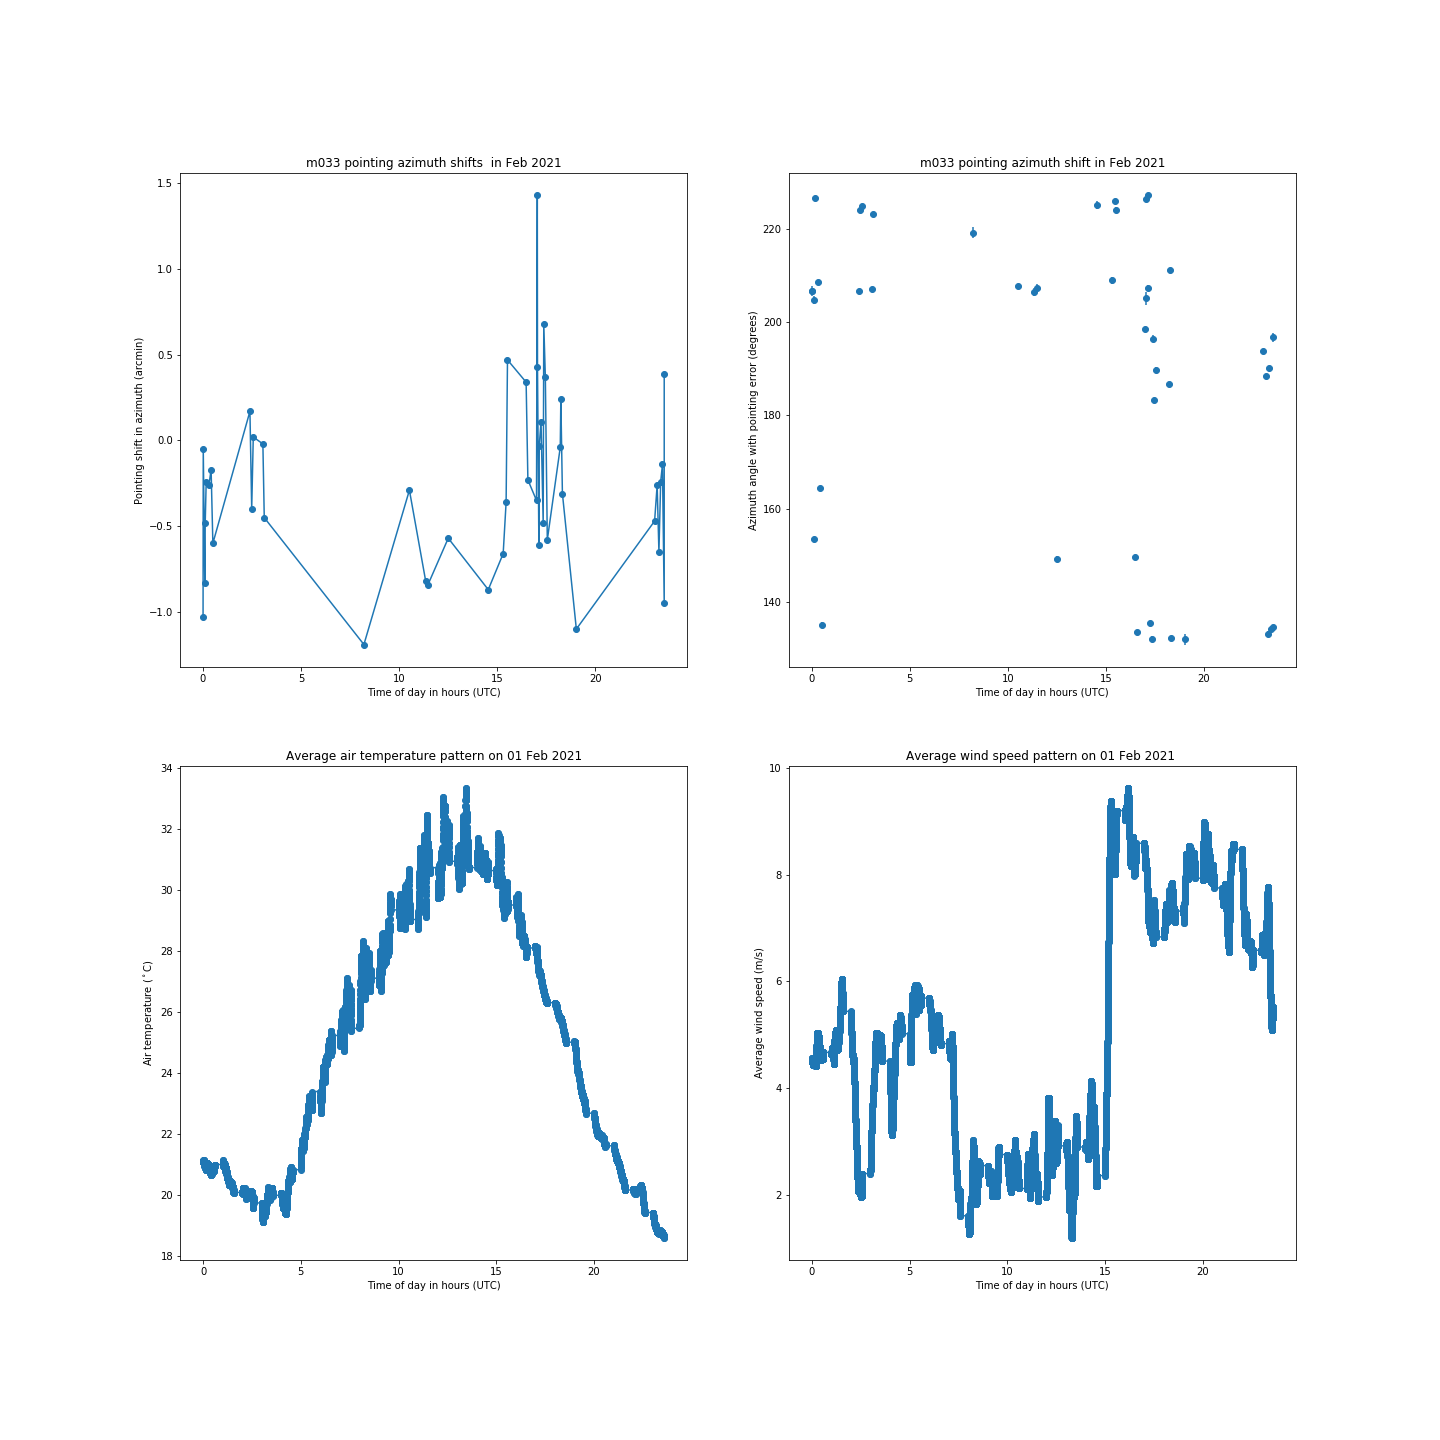
\includegraphics[scale=0.35]{m033_azim_Feb.png}
	
	%\includegraphics[resolution=100]{bur1.png}
	\caption{Plots of pointing error in azimuth, angle of azimuth, temperature and wind against time.}
	\label{fig:m033AzimFeb}
\end{figure}


\begin{figure}[H]
	\centering
	%\includegraphicsdpi{100}{}{bur1.png}     
	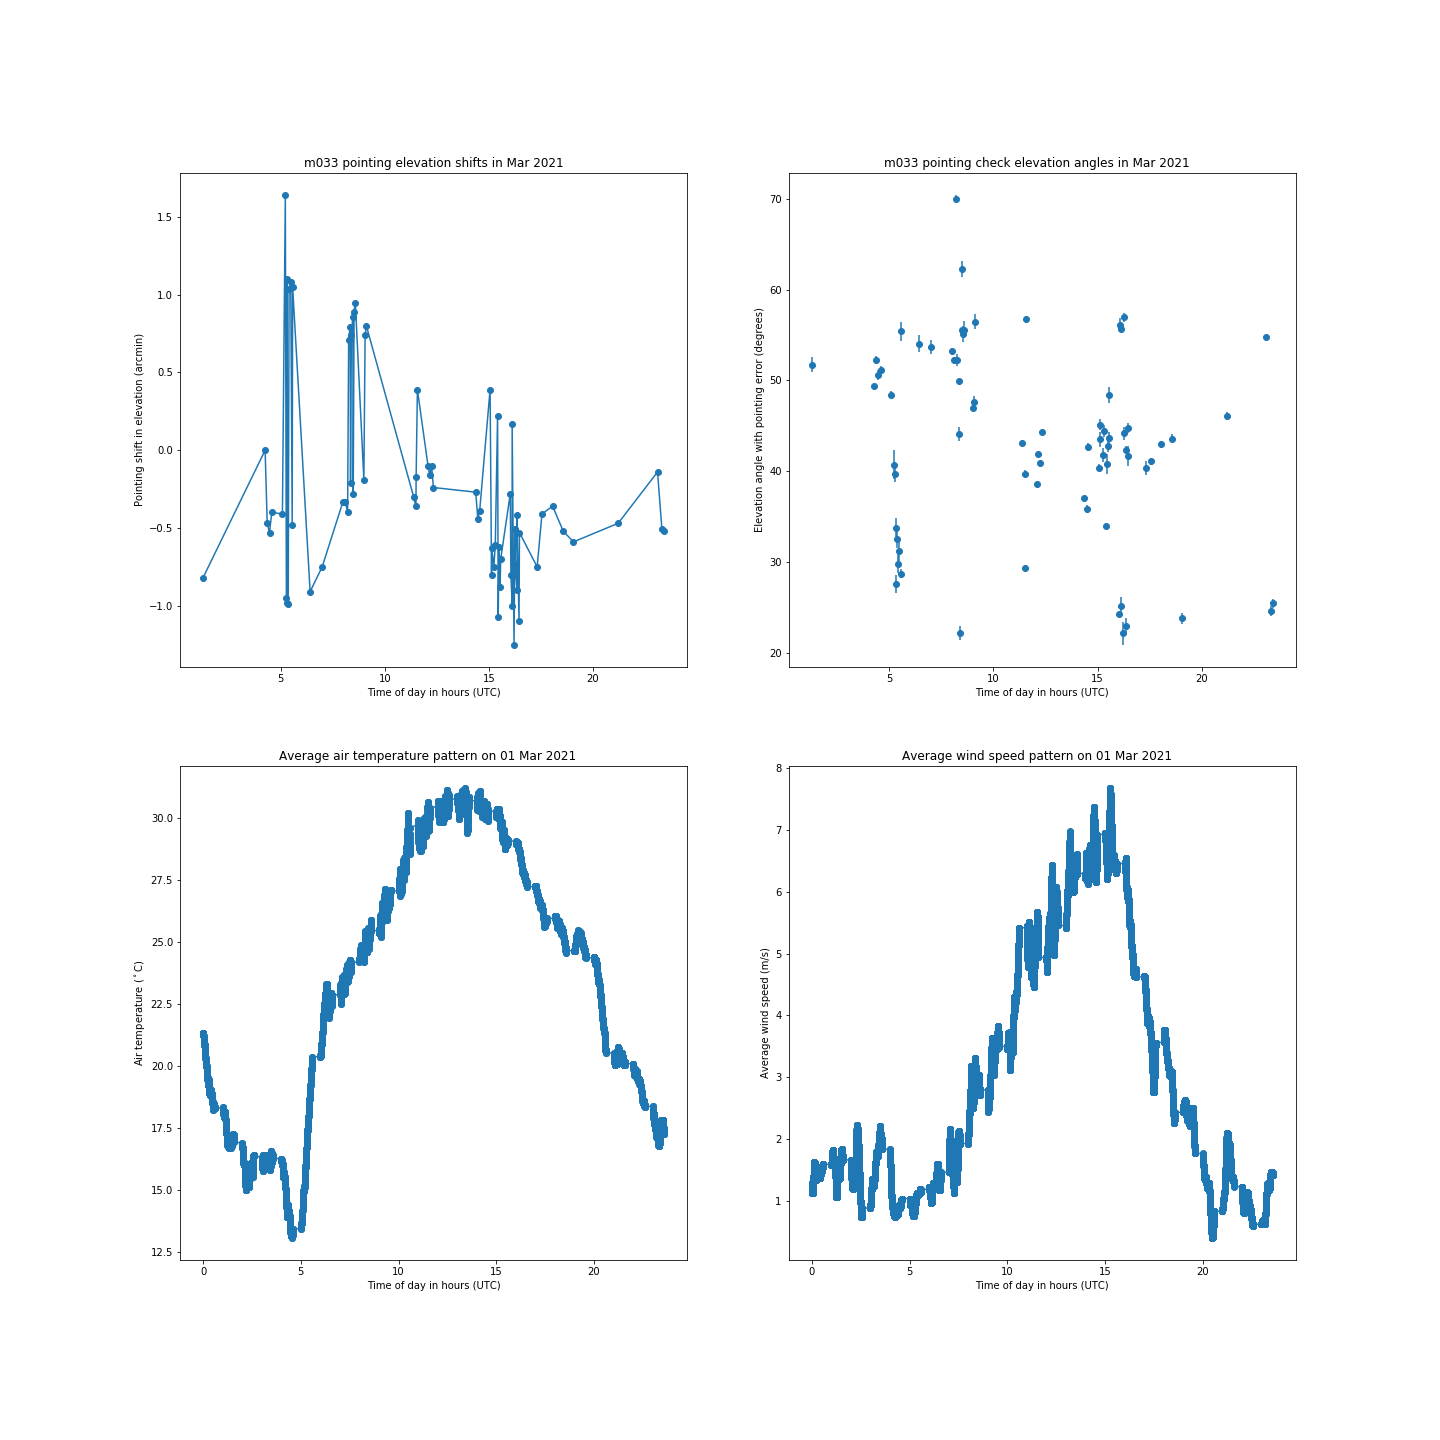
\includegraphics[scale=0.35]{m033_elev_Mar.png}
	
	%\includegraphics[resolution=100]{bur1.png}
	\caption{Plots of pointing error in elevation, angle of elevation, temperature and wind against time.}
	\label{fig:m033ElevMar}
\end{figure}

\begin{figure}[H]
	\centering
	%\includegraphicsdpi{100}{}{bur1.png}     
	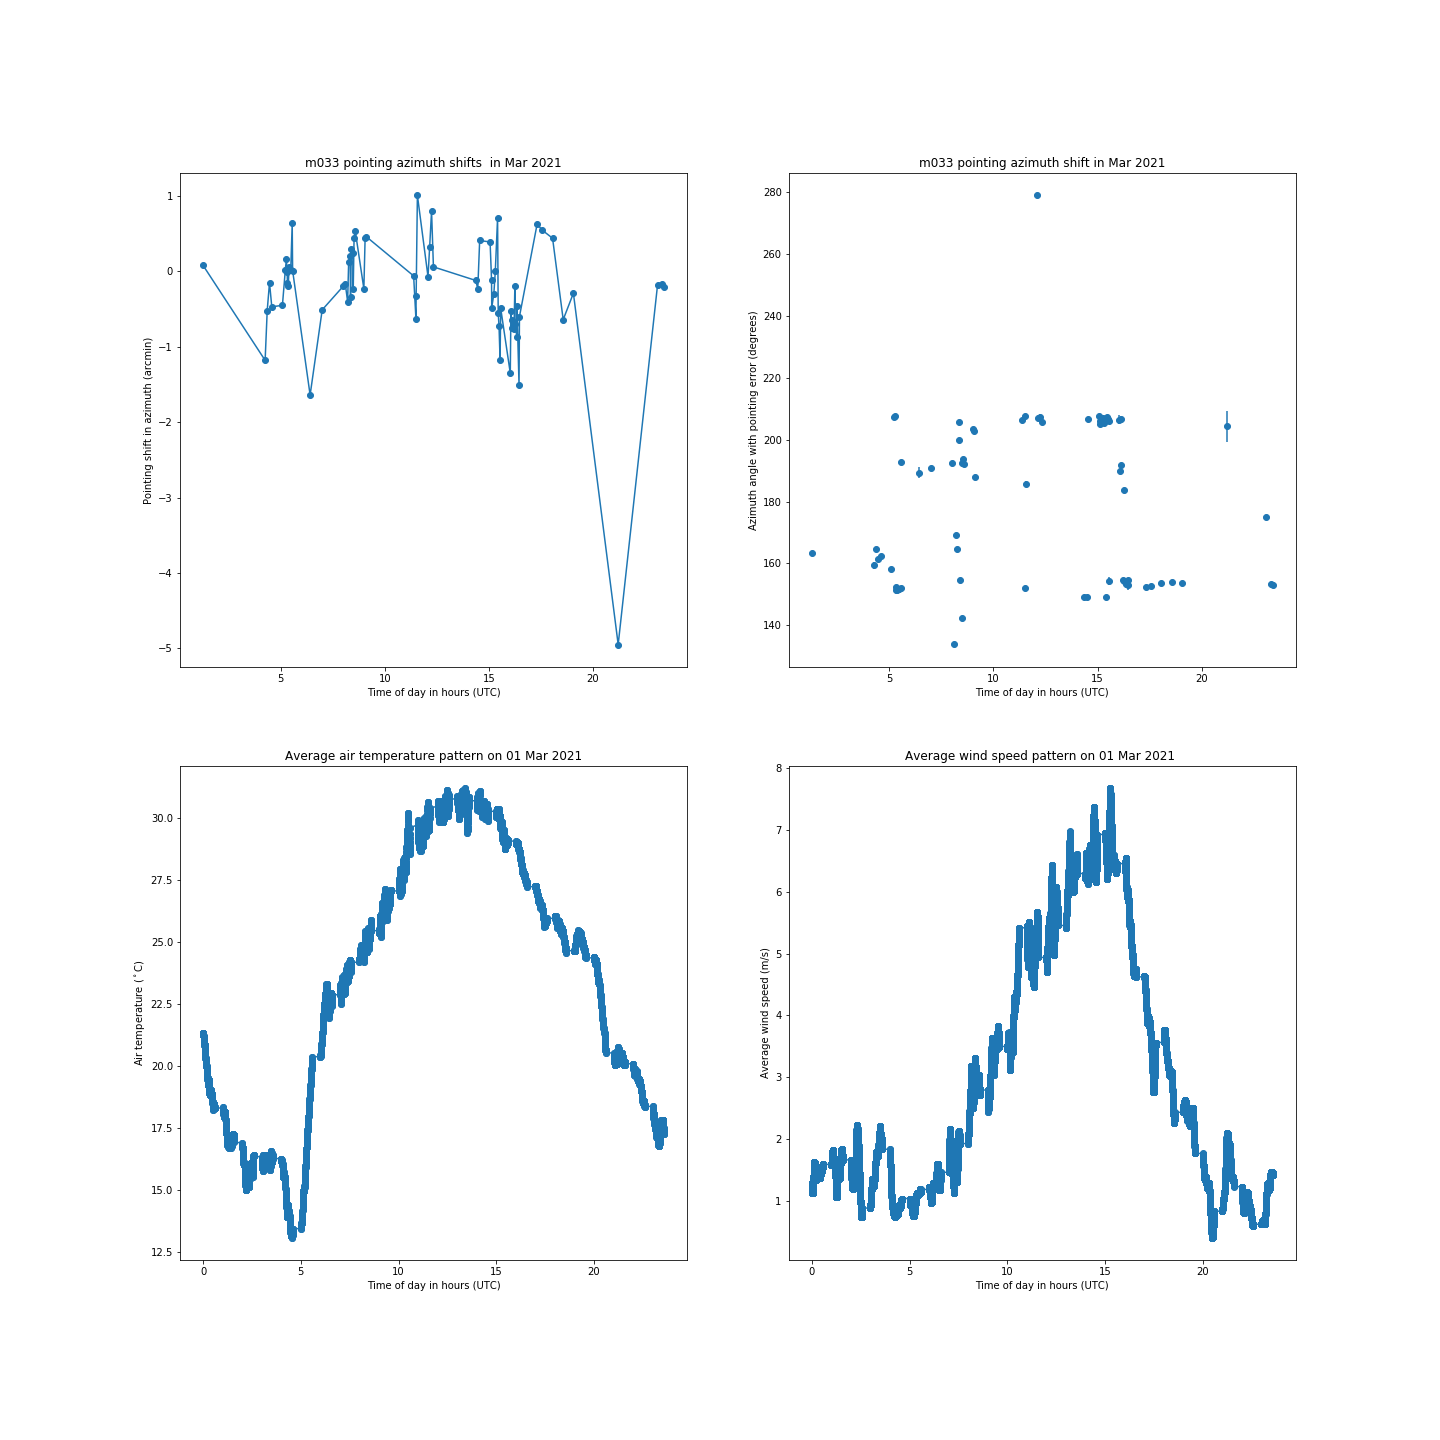
\includegraphics[scale=0.35]{m033_azim_Mar.png}
	
	%\includegraphics[resolution=100]{bur1.png}
	\caption{Plots of pointing error in azimuth, angle of azimuth, temperature and wind against time.}
	\label{fig:m033AzimMar}
\end{figure}


\begin{figure}[H]
	\centering
	%\includegraphicsdpi{100}{}{bur1.png}     
	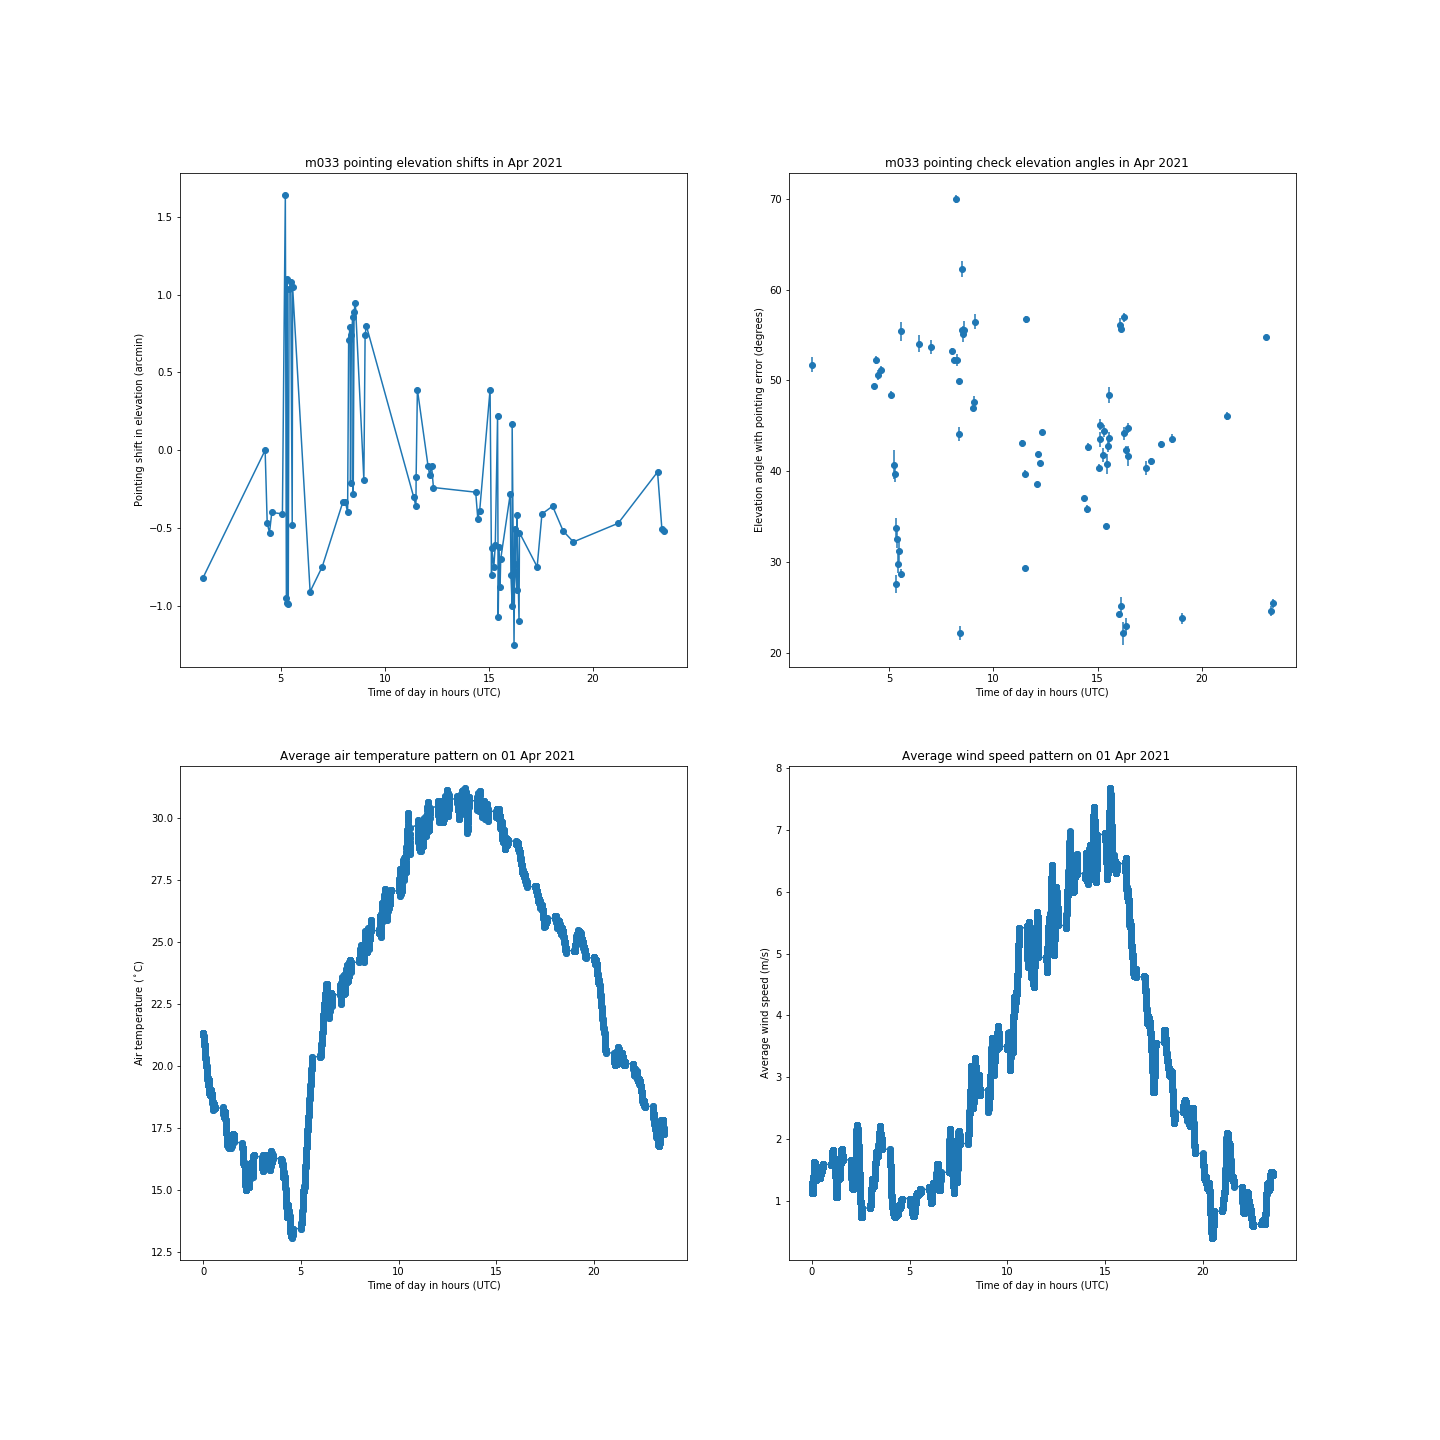
\includegraphics[scale=0.35]{m033_elev_Apr.png}
	
	%\includegraphics[resolution=100]{bur1.png}
	\caption{Plots of pointing error in elevation, angle of elevation, temperature and wind against time.}
	\label{fig:m033ElevApr}
\end{figure}

\begin{figure}[H]
	\centering
	%\includegraphicsdpi{100}{}{bur1.png}     
	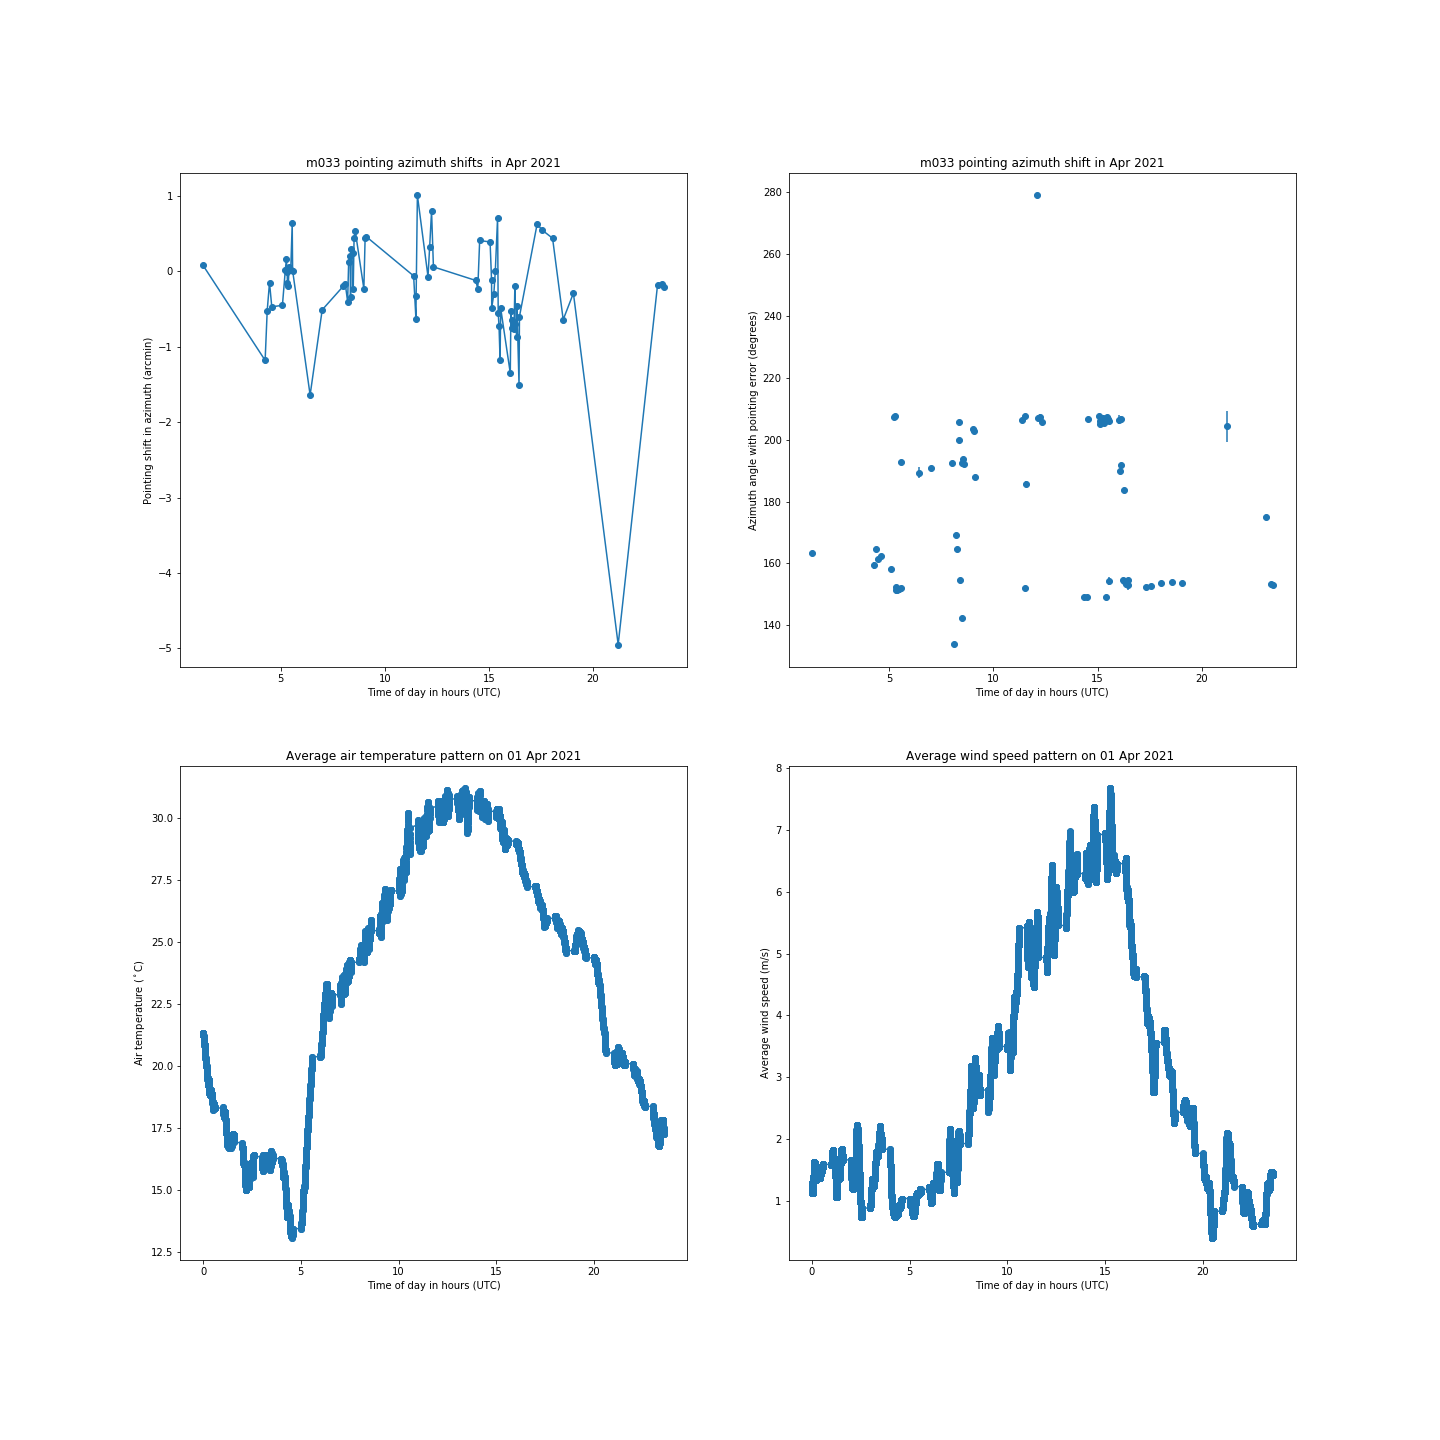
\includegraphics[scale=0.35]{m033_azim_Apr.png}
	
	%\includegraphics[resolution=100]{bur1.png}
	\caption{Plots of pointing error in azimuth, angle of azimuth, temperature and wind against time.}
	\label{fig:m033AzimApr}
\end{figure}

\begin{figure}[H]
	\centering
	%\includegraphicsdpi{100}{}{bur1.png}     
	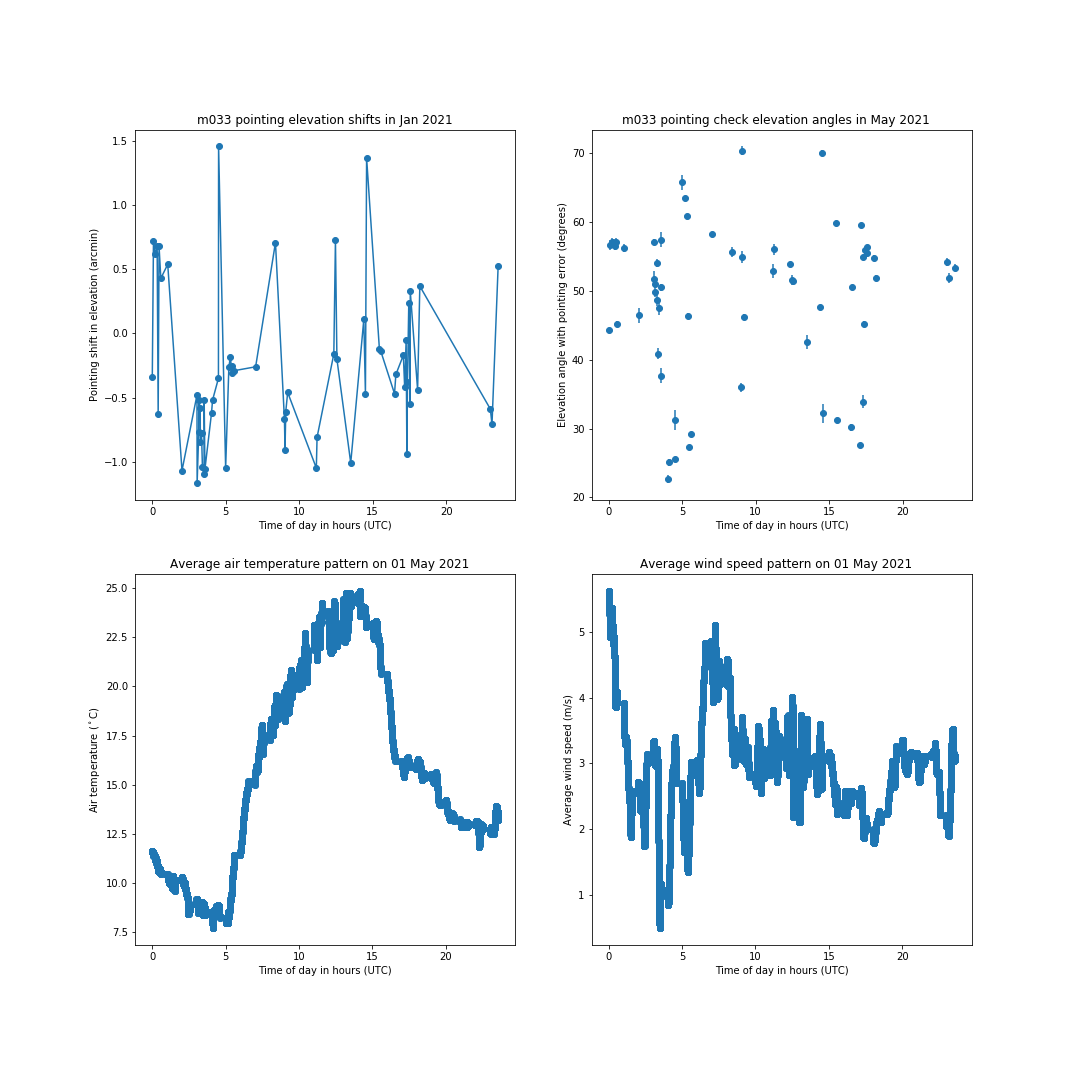
\includegraphics[scale=0.35]{m033_elev_May.png}
	
	%\includegraphics[resolution=100]{bur1.png}
	\caption{Plots of pointing error in elevation, angle of elevation, temperature and wind against time.}
	\label{fig:m033ElevMay}
\end{figure}

\begin{figure}[H]
	\centering
	%\includegraphicsdpi{100}{}{bur1.png}     
	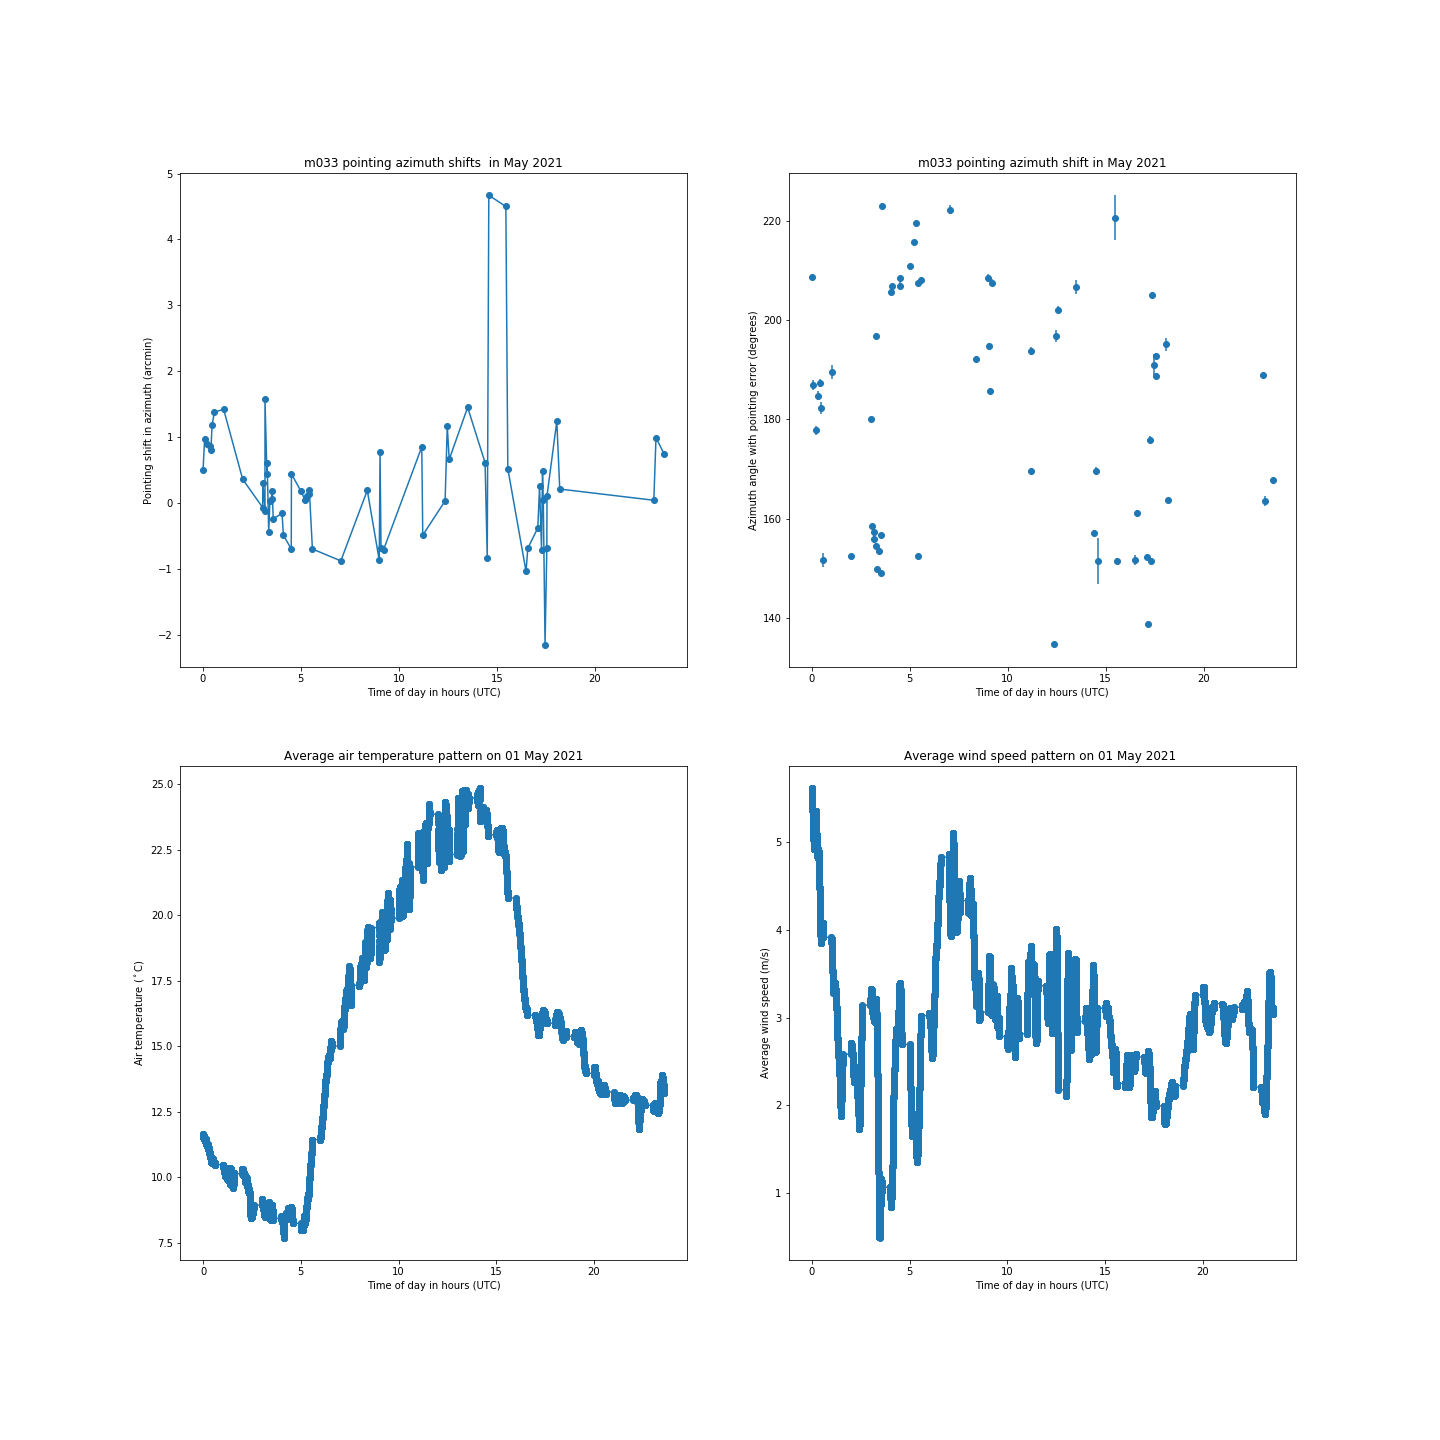
\includegraphics[scale=0.35]{m033_azim_May.png}
	
	%\includegraphics[resolution=100]{bur1.png}
	\caption{Plots of pointing error in azimuth, angle of azimuth, temperature and wind against time.}
	\label{fig:m033AzimMay}
\end{figure}


Similar to above plots, \textbf{Figure}~\ref{fig:m033ElevJanMapped} to \textbf{Figure}~\ref{fig:m033AzimMayMapped} show m033 pointing errors (adjustments) on the first row and, average temperature and wind during observation on the second row, all against time.    

\begin{figure}[H]
	%	\centering
	%\includegraphicsdpi{100}{}{bur1.png}     
	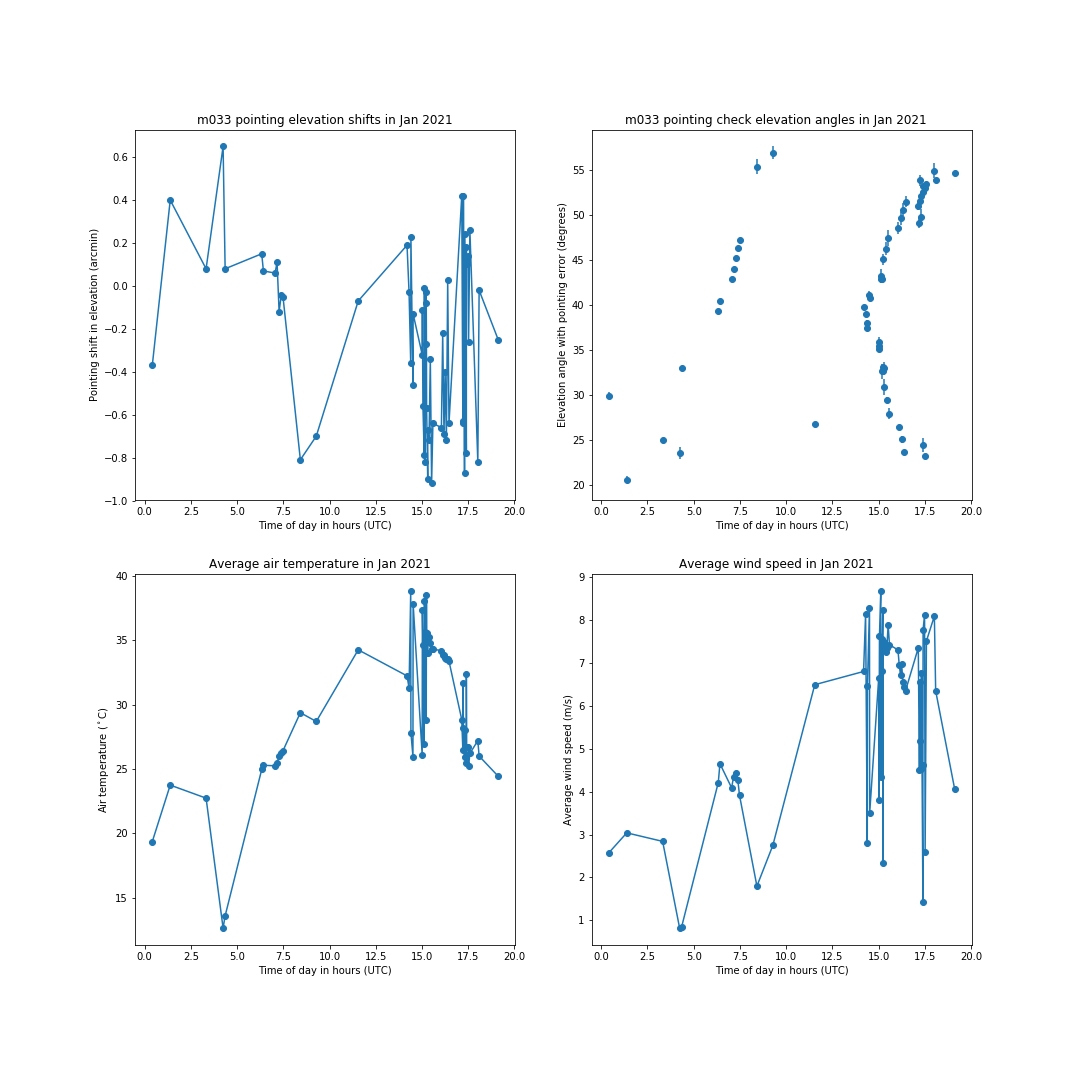
\includegraphics[scale=0.45]{m033_elev_Jan_mapped.png}
	
	%\includegraphics[resolution=100]{bur1.png}
	\caption{Plots of pointing error in elevation, angle of elevation, temperature and wind against time.}
	\label{fig:m033ElevJanMapped}
\end{figure}

\begin{figure}[H]
	\centering
	%\includegraphicsdpi{100}{}{bur1.png}     
	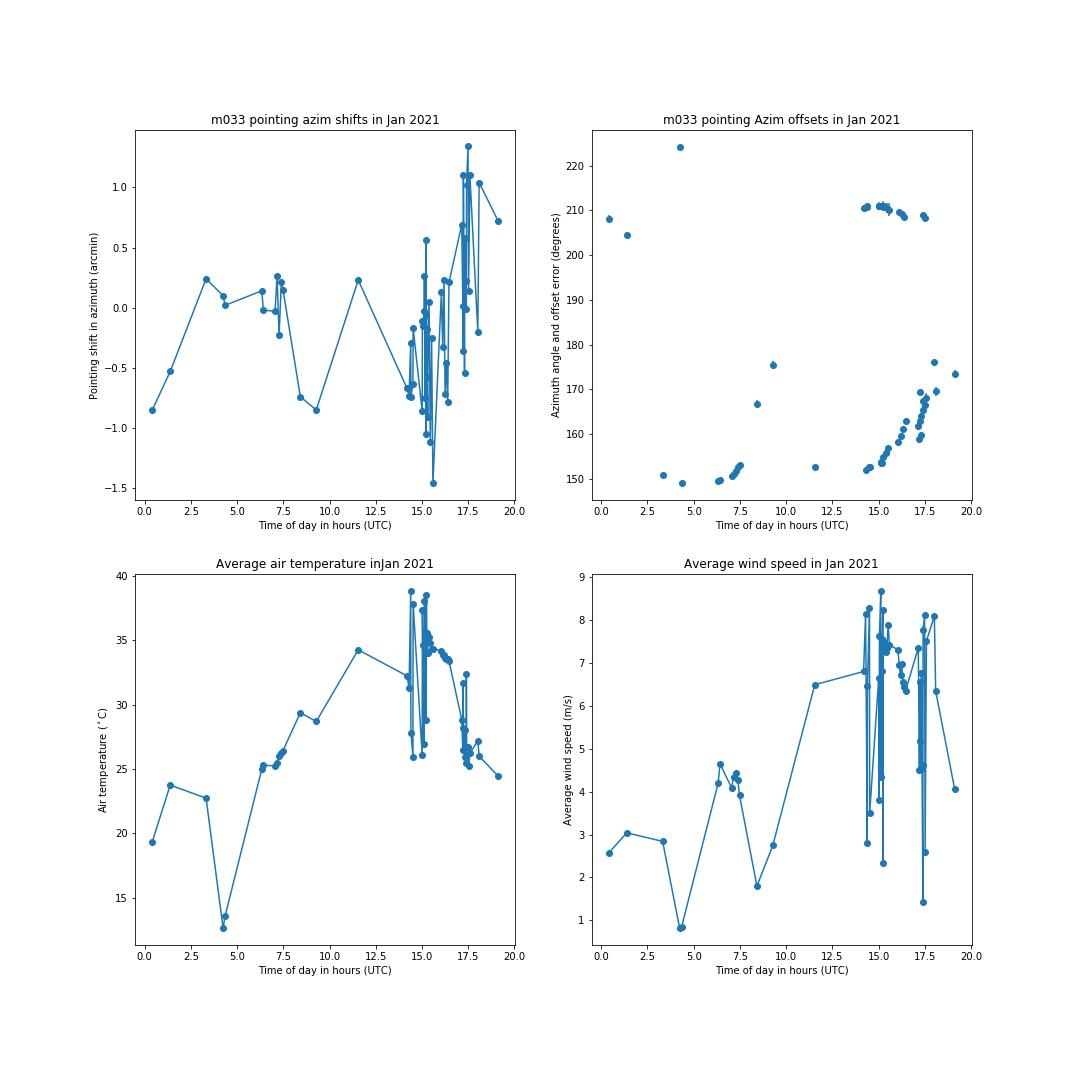
\includegraphics[scale=0.45]{m033_azim_Jan_mapped.png}
	
	%\includegraphics[resolution=100]{bur1.png}
	\caption{Plots of pointing error in azimuth, angle of azimuth, temperature and wind against time.}
	\label{fig:m033AzimJanMapped}
\end{figure}

\begin{figure}[H]
	\centering
	%\includegraphicsdpi{100}{}{bur1.png}     
	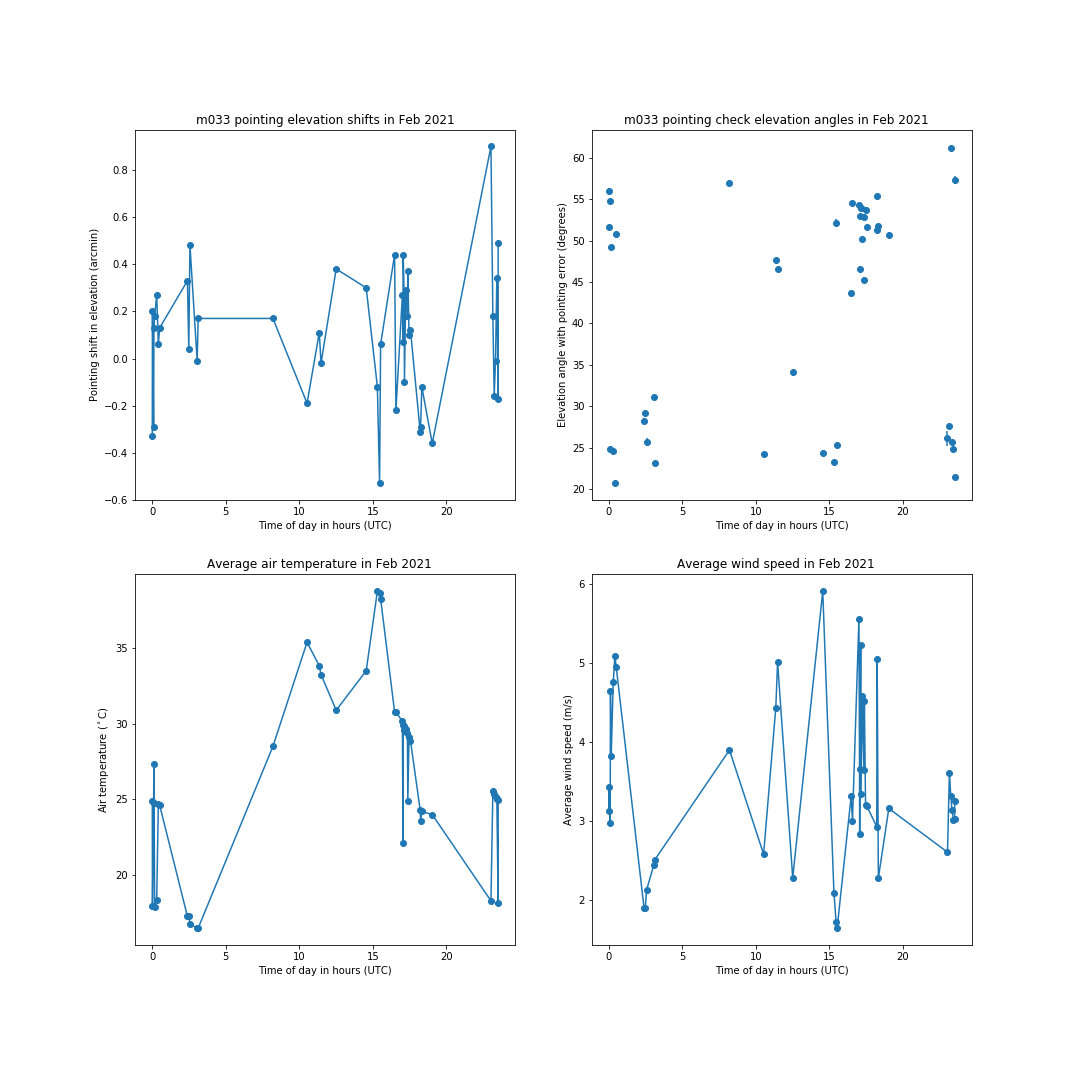
\includegraphics[scale=0.45]{m033_elev_Feb_mapped.png}
	
	%\includegraphics[resolution=100]{bur1.png}
	\caption{Plots of pointing error in elevation, angle of elevation, temperature and wind against time.}
	\label{fig:m033ElevFebMapped}
\end{figure}

\begin{figure}[H]
	\centering
	%\includegraphicsdpi{100}{}{bur1.png}     
	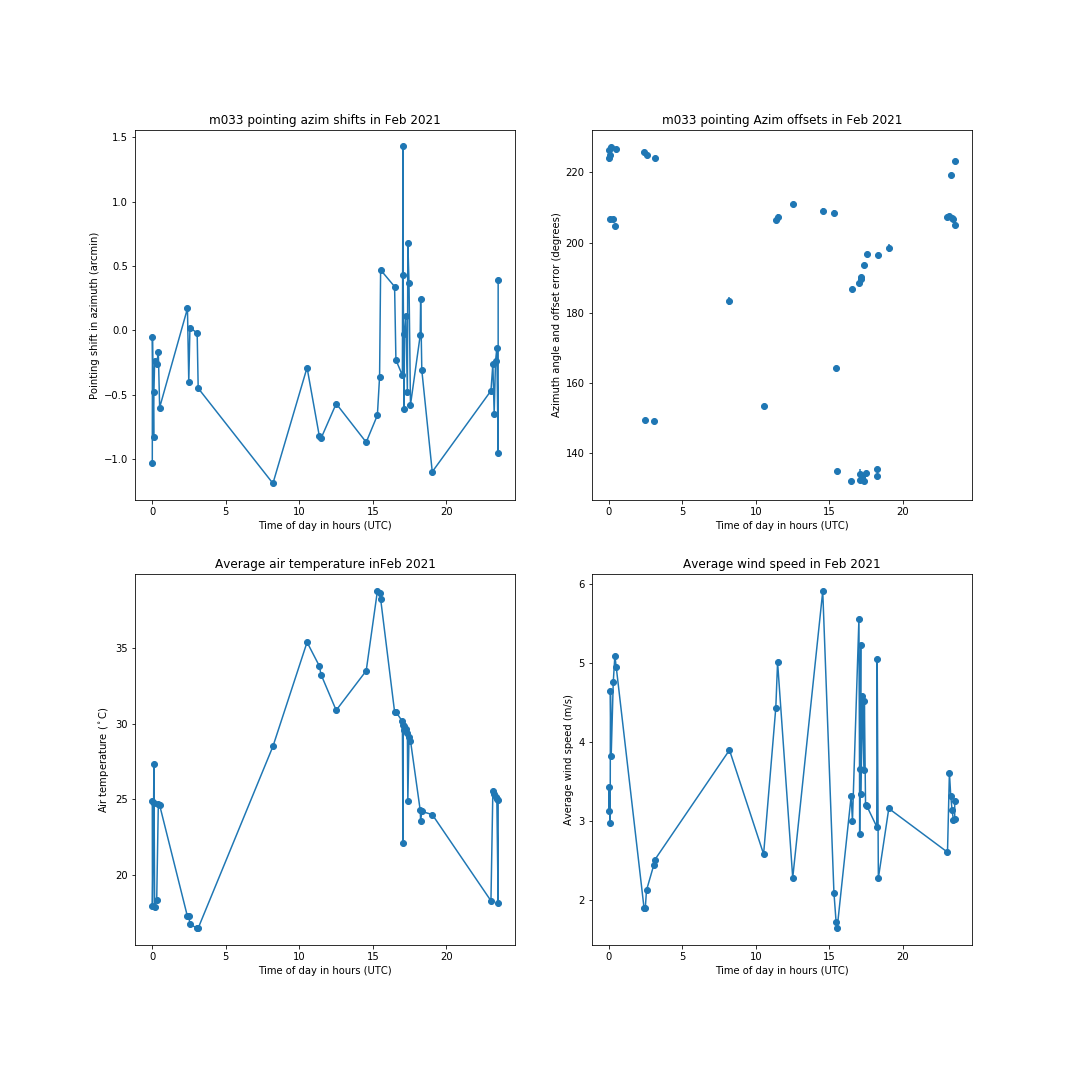
\includegraphics[scale=0.45]{m033_azim_Feb_mapped.png}
	
	%\includegraphics[resolution=100]{bur1.png}
	\caption{Plots of pointing error in azimuth, angle of azimuth, temperature and wind against time.}
	\label{fig:m033AzimFebMapped}
\end{figure}


\begin{figure}[H]
	\centering
	%\includegraphicsdpi{100}{}{bur1.png}     
	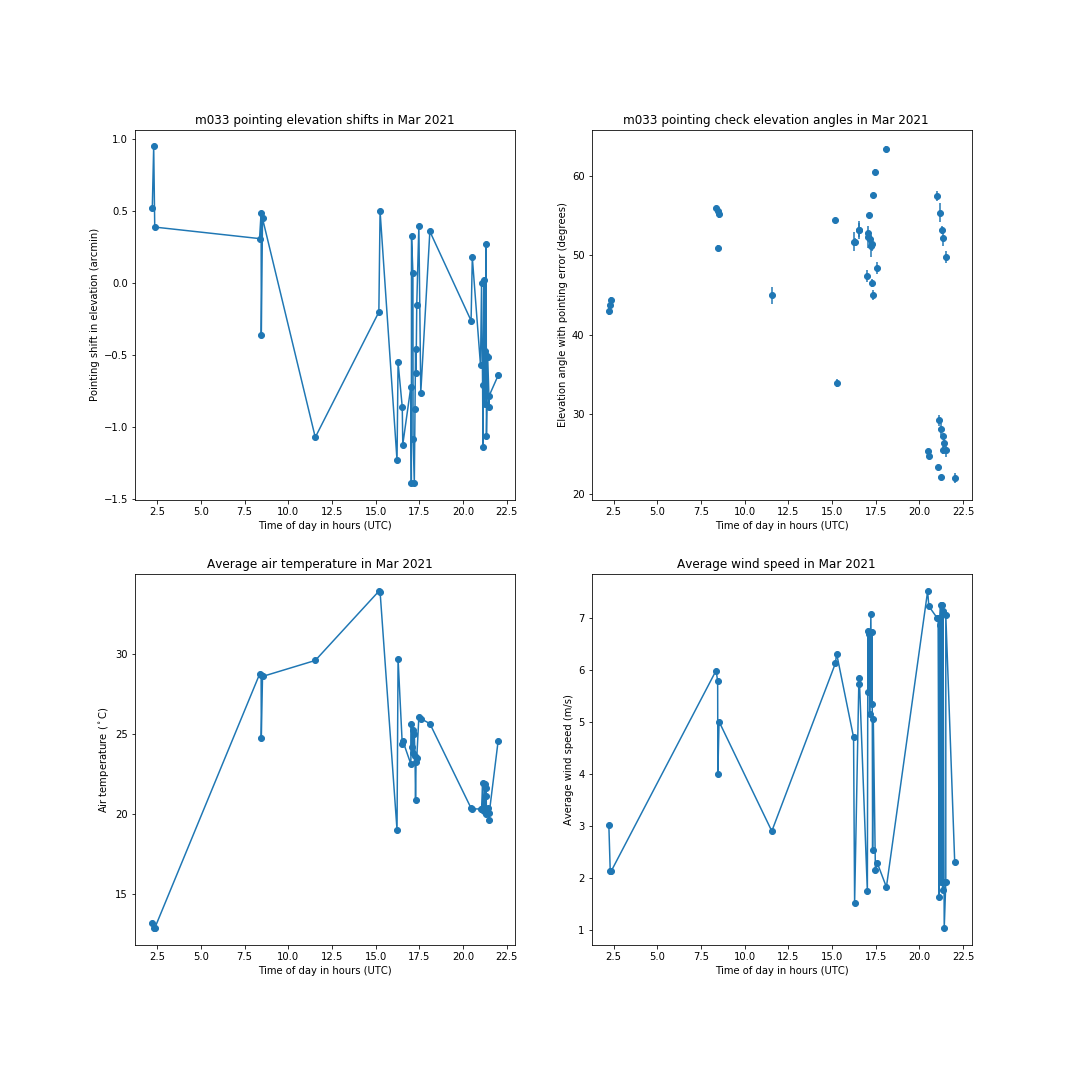
\includegraphics[scale=0.45]{m033_elev_Mar_mapped.png}
	
	%\includegraphics[resolution=100]{bur1.png}
	\caption{Plots of pointing error in elevation, angle of elevation, temperature and wind against time.}
	\label{fig:m033ElevMarMapped}
\end{figure}

\begin{figure}[H]
	\centering
	%\includegraphicsdpi{100}{}{bur1.png}     
	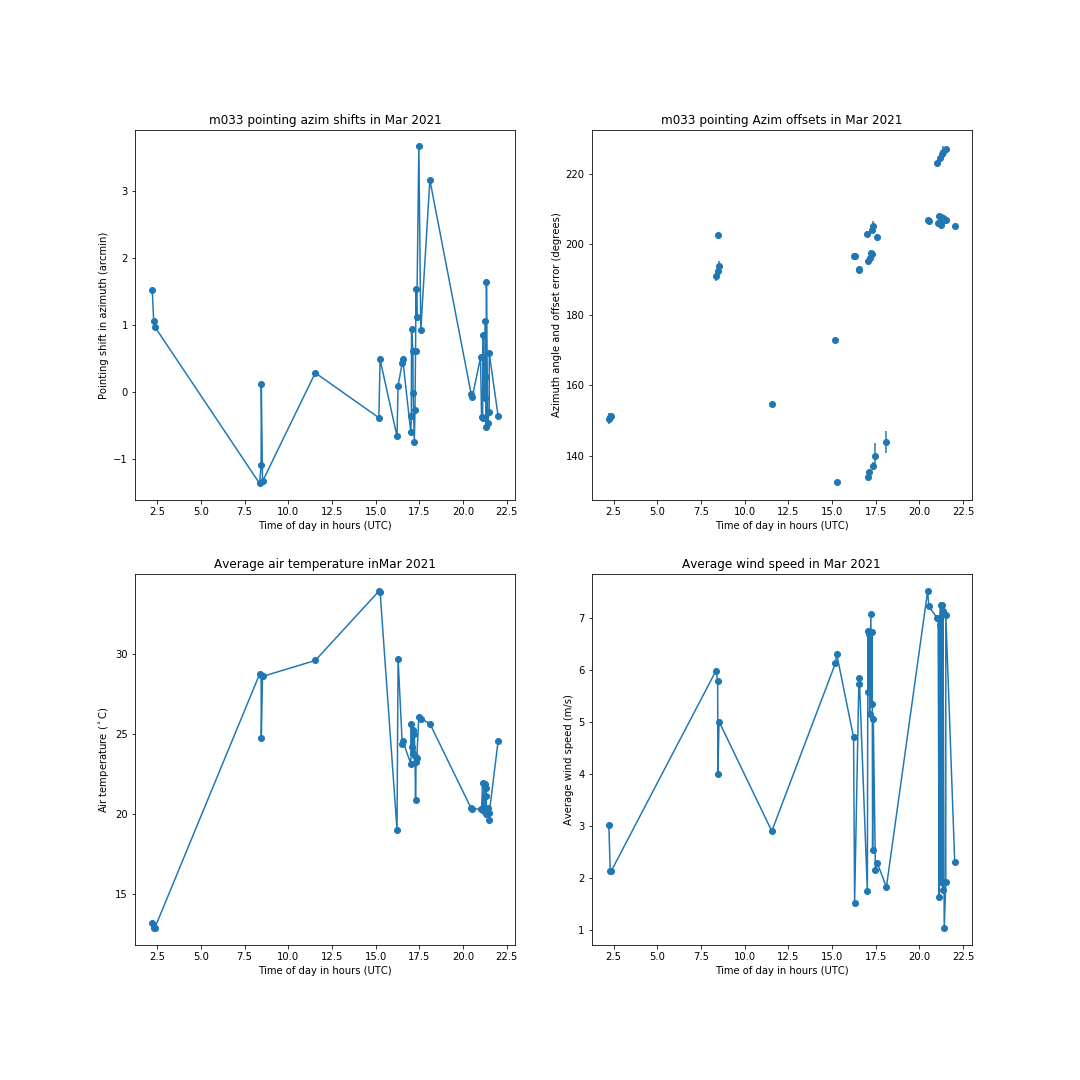
\includegraphics[scale=0.45]{m033_azim_Mar_mapped.png}
	
	%\includegraphics[resolution=100]{bur1.png}
	\caption{Plots of pointing error in azimuth, angle of azimuth, temperature and wind against time.}
	\label{fig:m033AzimMarMapped}
\end{figure}


\begin{figure}[H]
	\centering
	%\includegraphicsdpi{100}{}{bur1.png}     
	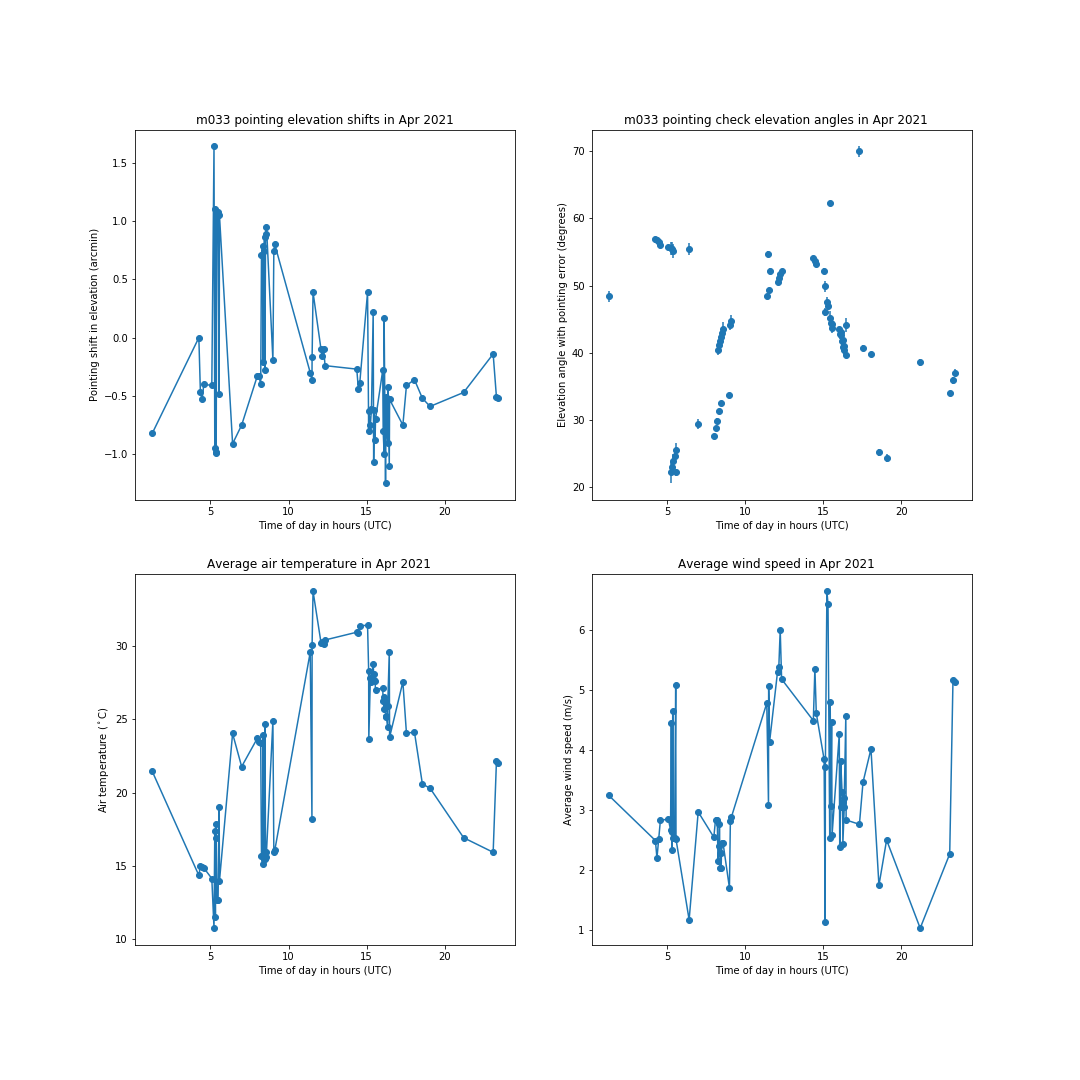
\includegraphics[scale=0.45]{m033_elev_Apr_mapped.png}
	
	%\includegraphics[resolution=100]{bur1.png}
	\caption{Plots of pointing error in elevation, angle of elevation, temperature and wind against time.}
	\label{fig:m033ElevAprMapped}
\end{figure}

\begin{figure}[H]
	\centering
	%\includegraphicsdpi{100}{}{bur1.png}     
	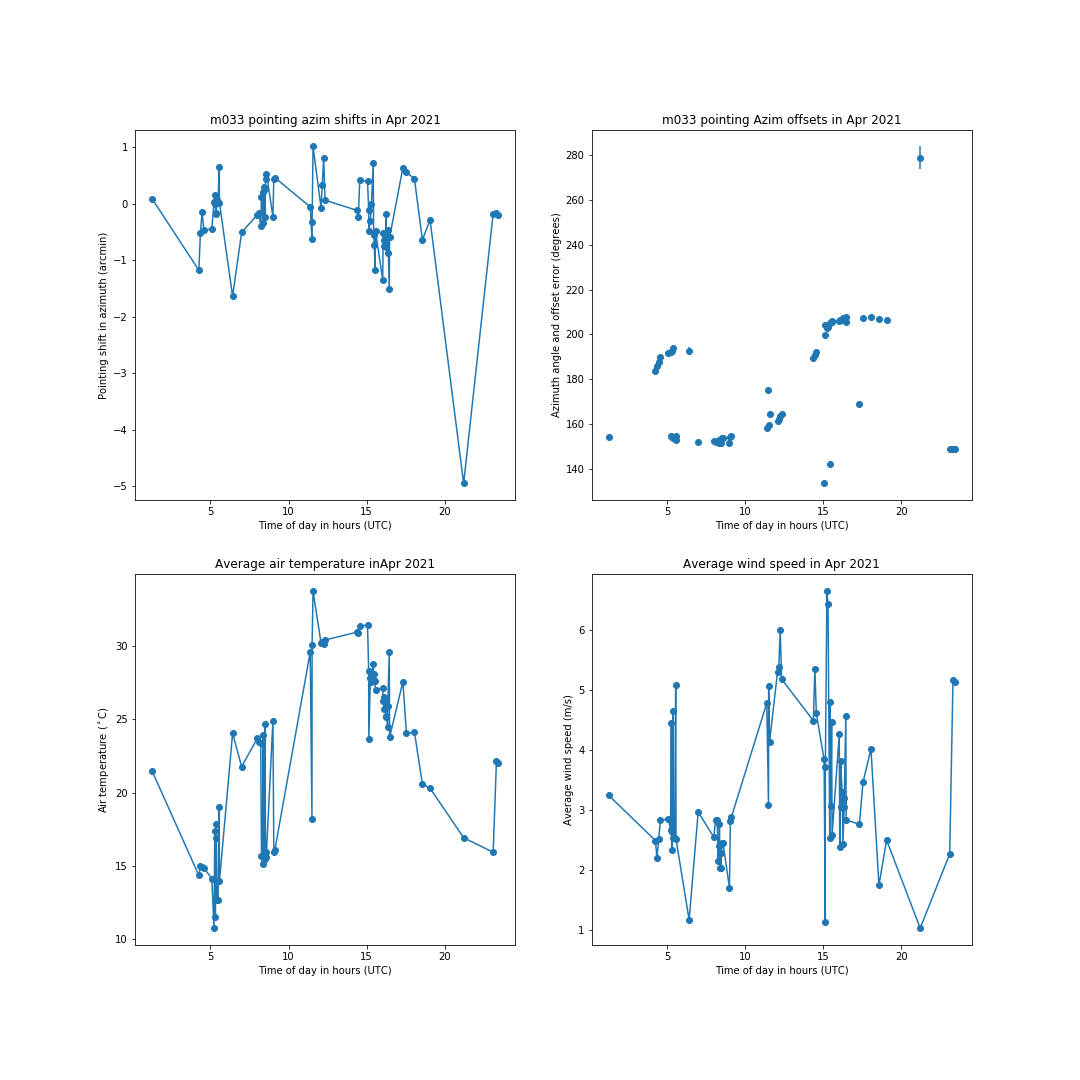
\includegraphics[scale=0.45]{m033_azim_Apr_mapped.png}
	
	%\includegraphics[resolution=100]{bur1.png}
	\caption{Plots of pointing error in azimuth, angle of azimuth, temperature and wind against time.}
	\label{fig:m033AzimAprMapped}
\end{figure}


\begin{figure}[H]
	\centering
	%\includegraphicsdpi{100}{}{bur1.png}     
	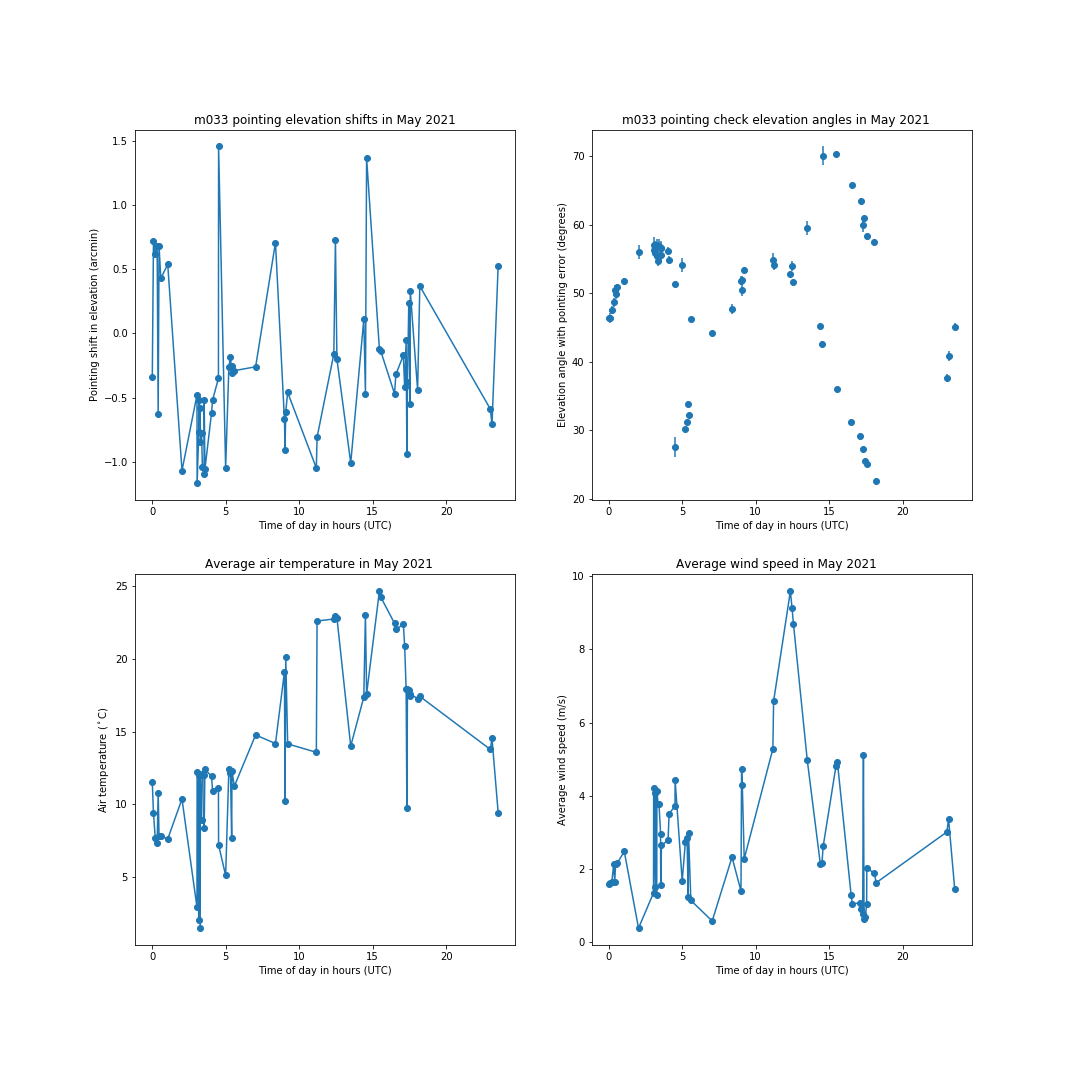
\includegraphics[scale=0.45]{m033_elev_May_mapped.png}
	
	%\includegraphics[resolution=100]{bur1.png}
	\caption{Plots of pointing error in elevation, angle of elevation, temperature and wind against time.}
	\label{fig:m033ElevMayMapped}
\end{figure}

\begin{figure}[H]
	\centering
	%\includegraphicsdpi{100}{}{bur1.png}     
	\includegraphics[scale=0.45]{m033_azim_May_mapped.png}
	
	%\includegraphics[resolution=100]{bur1.png}
	\caption{Plots of pointing error in azimuth, angle of azimuth, temperature and wind against time.}
	\label{fig:m033AzimMayMapped}
\end{figure}

\subsection{Antenna m009 Pointing Check Script Results  }
\begin{figure}[H]
	%	\centering
	%\includegraphicsdpi{100}{}{bur1.png}     
	\includegraphics[scale=0.45]{m009_elev_Jan.png}
	
	%\includegraphics[resolution=100]{bur1.png}
	\caption{Plots of pointing error in elevation, angle of elevation, temperature and wind against time.}
	\label{fig:m009ElevJan}
\end{figure}

\begin{figure}[H]
	\centering
	%\includegraphicsdpi{100}{}{bur1.png}     
	\includegraphics[scale=0.45]{m009_azim_Jan.png}
	
	%\includegraphics[resolution=100]{bur1.png}
	\caption{Plots of pointing error in azimuth, angle of azimuth, temperature and wind against time.}
	\label{fig:m009AzimJan}
\end{figure}

\begin{figure}[H]
	\centering
	%\includegraphicsdpi{100}{}{bur1.png}     
	\includegraphics[scale=0.45]{m009_elev_Feb.png}
	
	%\includegraphics[resolution=100]{bur1.png}
	\caption{Plots of pointing error in elevation, angle of elevation, temperature and wind against time.}
	\label{fig:m009ElevFeb}
\end{figure}

\begin{figure}[H]
	\centering
	%\includegraphicsdpi{100}{}{bur1.png}     
	\includegraphics[scale=0.45]{m009_azim_Feb.png}
	
	%\includegraphics[resolution=100]{bur1.png}
	\caption{Plots of pointing error in azimuth, angle of azimuth, temperature and wind against time.}
	\label{fig:m009AzimFeb}
\end{figure}


\begin{figure}[H]
	\centering
	%\includegraphicsdpi{100}{}{bur1.png}     
	\includegraphics[scale=0.45]{m009_elev_Mar.png}
	
	%\includegraphics[resolution=100]{bur1.png}
	\caption{Plots of pointing error in elevation, angle of elevation, temperature and wind against time.}
	\label{fig:m009ElevMar}
\end{figure}

\begin{figure}[H]
	\centering
	%\includegraphicsdpi{100}{}{bur1.png}     
	\includegraphics[scale=0.45]{m009_azim_Mar.png}
	
	%\includegraphics[resolution=100]{bur1.png}
	\caption{Plots of pointing error in azimuth, angle of azimuth, temperature and wind against time.}
	\label{fig:m009AzimMar}
\end{figure}


\begin{figure}[H]
	\centering
	%\includegraphicsdpi{100}{}{bur1.png}     
	\includegraphics[scale=0.45]{m009_elev_Apr.png}
	
	%\includegraphics[resolution=100]{bur1.png}
	\caption{Plots of pointing error in elevation, angle of elevation, temperature and wind against time.}
	\label{fig:m009ElevApr}
\end{figure}

\begin{figure}[H]
	\centering
	%\includegraphicsdpi{100}{}{bur1.png}     
	\includegraphics[scale=0.45]{m009_azim_Apr.png}
	
	%\includegraphics[resolution=100]{bur1.png}
	\caption{Plots of pointing error in azimuth, angle of azimuth, temperature and wind against time.}
	\label{fig:m009AzimApr}
\end{figure}

\begin{figure}[H]
	\centering
	%\includegraphicsdpi{100}{}{bur1.png}     
	\includegraphics[scale=0.45]{m009_elev_May.png}
	
	%\includegraphics[resolution=100]{bur1.png}
	\caption{Plots of pointing error in elevation, angle of elevation, temperature and wind against time.}
	\label{fig:m009ElevMay}
\end{figure}

\begin{figure}[H]
	\centering
	%\includegraphicsdpi{100}{}{bur1.png}     
	\includegraphics[scale=0.45]{m009_azim_May.png}
	
	%\includegraphics[resolution=100]{bur1.png}
	\caption{Plots of pointing error in azimuth, angle of azimuth, temperature and wind against time.}
	\label{fig:m009AzimMay}
\end{figure}
Similar to the above plots, \textbf{Figure}~\ref{fig:m009Elevmapped} to \textbf{Figure}~\ref{fig:m009AzimMarMapped}  m009 pointing errors (adjustments) on the first row and, average temperature and wind during observation on the second row, all against time.      

\begin{figure}[H]
	%	\centering
	%\includegraphicsdpi{100}{}{bur1.png}     
	\includegraphics[scale=0.45]{m009_elev_Jan_mapped.png}
	
	%\includegraphics[resolution=100]{bur1.png}
	\caption{Plots of pointing error in elevation, angle of elevation, temperature and wind against time.}
	\label{fig:m009ElevJanMapped}
\end{figure}

\begin{figure}[H]
	\centering
	%\includegraphicsdpi{100}{}{bur1.png}     
	\includegraphics[scale=0.45]{m009_azim_Jan_mapped.png}
	
	%\includegraphics[resolution=100]{bur1.png}
	\caption{Plots of pointing error in azimuth, angle of azimuth, temperature and wind against time.}
	\label{fig:m009AzimJanMapped}
\end{figure}

\begin{figure}[H]
	\centering
	%\includegraphicsdpi{100}{}{bur1.png}     
	\includegraphics[scale=0.45]{m009_elev_Feb_mapped.png}
	
	%\includegraphics[resolution=100]{bur1.png}
	\caption{Plots of pointing error in elevation, angle of elevation, temperature and wind against time.}
	\label{fig:m009ElevFebMapped}
\end{figure}

\begin{figure}[H]
	\centering
	%\includegraphicsdpi{100}{}{bur1.png}     
	\includegraphics[scale=0.45]{m009_azim_Feb_mapped.png}
	
	%\includegraphics[resolution=100]{bur1.png}
	\caption{Plots of pointing error in azimuth, angle of azimuth, temperature and wind against time.}
	\label{fig:m009AzimFebMapped}
\end{figure}


\begin{figure}[H]
	\centering
	%\includegraphicsdpi{100}{}{bur1.png}     
	\includegraphics[scale=0.45]{m009_elev_Mar_mapped.png}
	
	%\includegraphics[resolution=100]{bur1.png}
	\caption{Plots of pointing error in elevation, angle of elevation, temperature and wind against time.}
	\label{fig:m009ElevMarMapped}
\end{figure}

\begin{figure}[H]
	\centering
	%\includegraphicsdpi{100}{}{bur1.png}     
	\includegraphics[scale=0.45]{m009_azim_Mar_mapped.png}
	
	%\includegraphics[resolution=100]{bur1.png}
	\caption{Plots of pointing error in azimuth, angle of azimuth, temperature and wind against time.}
	\label{fig:m009AzimMarMapped}
\end{figure}


\begin{figure}[H]
	\centering
	%\includegraphicsdpi{100}{}{bur1.png}     
	\includegraphics[scale=0.45]{m009_elev_Apr_mapped.png}
	
	%\includegraphics[resolution=100]{bur1.png}
	\caption{Plots of pointing error in elevation, angle of elevation, temperature and wind against time.}
	\label{fig:m009ElevAprMapped}
\end{figure}

\begin{figure}[H]
	\centering
	%\includegraphicsdpi{100}{}{bur1.png}     
	\includegraphics[scale=0.45]{m009_azim_Apr_mapped.png}
	
	%\includegraphics[resolution=100]{bur1.png}
	\caption{Plots of pointing error in azimuth, angle of azimuth, temperature and wind against time.}
	\label{fig:m009AzimAprMapped}
\end{figure}


\begin{figure}[H]
	\centering
	%\includegraphicsdpi{100}{}{bur1.png}     
	\includegraphics[scale=0.45]{m009_elev_May_mapped.png}
	
	%\includegraphics[resolution=100]{bur1.png}
	\caption{Plots of pointing error in elevation, angle of elevation, temperature and wind against time.}
	\label{fig:m009ElevMayMapped}
\end{figure}

\begin{figure}[H]
	\centering
	%\includegraphicsdpi{100}{}{bur1.png}     
	\includegraphics[scale=0.45]{m009_azim_May_mapped.png}
	
	%\includegraphics[resolution=100]{bur1.png}
	\caption{Plots of pointing error in azimuth, angle of azimuth, temperature and wind against time.}
	\label{fig:m009AzimMayMapped}
\end{figure}
\subsection{Correlation Between Temperature and Pointing Error }
Correlations between temeperature and pointing error in both elevation and azimuth is shown in \textbf{Table}~\ref{tab:table1} and \textbf{Table}~\ref{tab:table3}. Futhermore, correlations between wind and pointing errors in both elevation and azimuth are shown in \textbf{Table}~\ref{tab:table2} \textbf{Table}~\ref{tab:table4}.  Since pointing errors can either be negative or positive depending on the direction of shift from the offset, correlations between wind/temperature and absolute values of the errors are also included in the table.
\begin{table}[H]
	\caption{Correlation between temperature and pointing error on m009}
	\label{tab:table1}
	\centering	
	\begin{tabular}[b]{|c|c|c|c|c|c|}
		\hline
		&\textbf{Jan}	& \textbf{Feb}& \textbf{Mar}&\textbf{Apr}&\textbf{May}\\
		\hline
		Cor (with negative elev values) &-0,49&-0.39&0.9&0.21&0.20\\
		\hline
		Cor (with absolute elev values) &-0.04&-0.23&0.11&0.01&0.04\\
		\hline
		Cor (with negative azim values) &-0.19&-0.29&0.20&0.38&0.42\\	
		\hline
		Cor (with absolute azim values) &0.08&0.23&0.01&0.24&0.20\\	
		\hline
	\end{tabular}	
\end{table}
\begin{table}[H]
	\caption{Correlation between temperature and pointing error on m033}
	\label{tab:table2}
	\centering	
	\begin{tabular}[b]{|c|c|c|c|c|c|}
		\hline
		&\textbf{Jan}	& \textbf{Feb}& \textbf{Mar}&\textbf{Apr}&\textbf{May}\\
		\hline
		Cor (with negative elev values) &-0.39&-0.22&-0.04&0.21&0.04\\
		\hline
		Cor (with absolute elev values) &0.13&-0.08&-0.06&0.01&-0.37\\
		\hline
		Cor (with negative azim values) &-0.00&-0.10&-0.19&0.38&-0.03\\	
		\hline
		Cor (with absolute azim values) &0.02&0.18&-0.19&0.24&0.25\\	
		\hline
	\end{tabular}	
\end{table}
\subsection{Correlation Between Wind Speed and Pointing Shift }

\begin{table}[H]
	\caption{Correlation between wind speed and pointing error on m009}
	\label{tab:table3}
	\centering	
	\begin{tabular}[b]{|c|c|c|c|c|c|}
		\hline
		&\textbf{Jan}	& \textbf{Feb}& \textbf{Mar}&\textbf{Apr}&\textbf{May}\\
		\hline
		Cor (with negative elev values) &-0.25&-0.06&-0.24&0.26&0.25\\
		\hline
		Cor (with absolute elev values) &-0.01&-0.02&-0.21&0.35&0.05\\
		\hline
		Cor (with negative azim values) &-0.18&-0.29&-0.16&-0.14&0.27\\	
		\hline
		Cor (with absolute azim values) &0.06&-0.09&0.01&-0.13&0.26\\	
		\hline
	\end{tabular}	
\end{table}

\begin{table}[H]
	\caption{Correlation between wind speed and pointing error on m033}
	\label{tab:table4}
	\centering	
	\begin{tabular}[b]{|c|c|c|c|c|c|}
		\hline
		&\textbf{Jan}	& \textbf{Feb}& \textbf{Mar}&\textbf{Apr}&\textbf{May}\\
		\hline
		Cor (with negative elev values) &-0.21&0.15&-0.12&0.25&-0.05\\
		\hline
		Cor (with absolute elev values) &0.13&-0.13&-0.04&0.01&0.15\\
		\hline
		Cor (with negative azim values) &-0.18&-0.12&-0.19&0.40&0.24\\	
		\hline
		Cor (with absolute azim values) &0.41&0.18&-0.19&-0.12&0.07\\
		\hline
	\end{tabular}
\end{table}
\section{Analysis of Data}

\subsection{Effects of Temperature and Wind on pointing Accuracy}
Observations of average wind speed and temperature over a month reveals that wearther patterns at site are predictable as shown in \textbf{Figure}~\ref{fig:wind1} and \textbf{Figure}~\ref{fig:temp1} respectively.  For most of the days in summer, air temperature reaches maximum values between 10:00 and 14:00 UTC, and minimum values between 02:00 and 05:00 UTC.  On average, wind speeds are lowest in the mornings between 02:00 and 05:00 UTC and highest in the evening.\\

A full day wind and temerature pattern is shown in figure \textbf{Figure}~\ref{fig:m033ElevJan} where the first day of Jan 2021 is chosen as a sample.  In this plot, pointing errors in elevation of antenna m033 are plotted against time of the day (i.e from 00:00 hour to 23:59 UTC).  A pointing error of  less than $|-1|$ is generally acceptable and do not require further adjustment of the pointing model.  In the plot, all elevation errors are less than $|-1|$ which implies that the errors are within the required range.  However, it is observed that most of the elevation error values closer to $|-1|$ occur between 16:00 UTC and 23:00.  This observation corresponds to increasing wind speeds with temperature beginning to drop.  A plot of m033 azimuth pointing errors is shown in \textbf{Figure}~\ref{fig:m033AzimJan}.  Similar to elevation errors, most higher values appear after 15:00, but with more values greater than $|-1|$. This implies that the effects of wind speed on azimuth pointing accuracy is more servere than on elevation accuracy.  Observations from Mar 2021 reveals an increase in both elevation and azimuth errors as illustrated in \textbf{Figure}~\ref{fig:m033ElevMar} to \textbf{Figure}~\ref{fig:m033AzimMay}.   \\


Antenna m009 pointing data was colected for comparison with m033 data.  It is evident from \textbf{Figure}~\ref{fig:m009ElevJan} to \textbf{Figure}~\ref{fig:m009AzimMay} the same argument for m033 applies for m009.  However, m009 pointing errors appears to slighlty more than that of m033.  \\


The exact wind speed and temperature during pointing observations is plotted agaist time of the day in \textbf{Figure}~\ref{fig:m033ElevJanMapped} to \textbf{Figure}~\ref{fig:m033AzimMayMapped} with antenna m033 pointing errors.  And similarly for antenna m009 in \textbf{Figure}~\ref{fig:m009ElevJanMapped} to \textbf{Figure}~\ref{fig:m009AzimMayMapped}.  It is evident from figures that many extreme pointing errors correspond to high wind speed.  There is also a possibilty that wind gusts at the time of observations were higher than the mean values. A clear demostration of the effects of wind on azimuth pointing error is shown in \textbf{Figure}~\ref{fig:m033AzimMayMapped} as azimuth errors reached values greater tha 4 arcmins.  Even though it was observed that the residual pointing error in elevation of the 40 m radio telescope
administered by Yunnan Observatories  is significantly higher than in
azimuth, which is possibly caused by temperature, wind {\cite{kong}, the Meerkat Telescope dish appears to be affected more in azimuth.   This could be attributed to the horizontal structures that holds the secondary reflector.  \\
	
	Calculations of correlations between wind/temperature and pointing error as shown on the \textbf{Table}~\ref{tab:table1} to \textbf{Table}~\ref{tab:table4} does not reveal convincing results.   The obious  reason is that solar illumination changes the whole day with the antenna structure bending in different dirrections, thus shifting pointing accuracy in different direction.  Furthermore, wind blows in different directions and also the antenna can point at different direction, thus the effects of wind can shift pointing accuracy in any dirrection.  
	
	
	\subsection{Faulty Components}
	Some of the MeerKat pointing issues were  caused by elevation and azimuth encoder slipages, encoder offset errors, encoder failures and tiltmeter errors.  Pointing errors due these fators are easily noticable as they show large drifts in pointing as shown in \textbf{Figure}~\ref{fig:m009ElevAprMapped} and \textbf{Figure}~\ref{fig:m009AzimAprMapped} 
	
	\subsection{Pointing Model Deficiencies - Temperature and Wind factors}
	
	According to the study \cite{Bayley}, temperature and wind are the most significant factors in pointing models.  Thus, to model the 32-m Merlin telescope, a number thermocouples were mounted on different metal beams of the antenna structures.  It was observed that a temperature difference of $6^\circ$C  caused a elevation offset of 10 arc sec.  Summer temperature at the MeerKat site can rise from $20.9^\circ$C to $44.9^\circ$C and winter temperatures from $10^\circ$C to $27^\circ$C. Nevertheless, the existing modeling of solar illumination seems to be effective since most pointing error values from sun rise to the maximum temperatures are within acceptable range.\\
	
	
	
	Tilts caused by differential heating from solar illumination can reach values up to about 50 arcseconds ( depending on the temperature and wind) \cite{Tony}.  The tilt meters are still under active investigation  \cite{SE}.  It was obvserved in this study that azimuth errors can reach values above 4 arcmins under high winds.  This suggest that the existing pointing model can handle Tilts caused by differential heating from solar illumination, physical structure deformations and tropospheric refraction much better, but wind remains a major challenge. 
	
	
	
	
	\section{Conclusion}
	There are many reported issues that are cuased by faulty components, especially ecoder slipping and tilt meter errors. Futhermore, there seems to be problems with current model with repect to how it models temperature and wind.  It was shown how a small change temperature in europe
	
	\clearpage
	
	\bibliographystyle{plain}
	\bibliography{references}
	\clearpage
\section{Appendix}
\appendix
\begin{appendices}
\section{JIRA MKAIV-487 Investigation -Single dish pointing approach  }\label{sec.py1}
\subsection{Introduction}
From all the basic functionality reports(Obs report) after the 21 Jan 2017, m025 had pointing errors.  Thus, m025 could not phase-up since then.  The last good basic functionality pointing report with m025 in the array was on the 18 Jan 2017(Good pointing report).  This was before the antenna got disconnected that afternoon(JIRA:MKAIV-487).   

\subsection{M025 status before disconnection on the 18 Jan 2017:}
\begin{itemize}
\item Disconnection sensors.  
\begin{figure}[H]
	\centering
	%\includegraphicsdpi{100}{}{bur1.png}     
	\includegraphics[scale=0.33]{m025_investigate.png}
	
	%\includegraphics[resolution=100]{bur1.png}
	\caption{Tilt meter disconnect error}
	\label{fig:tilt1}
\end{figure}


\item Basic Functionality Pointing report before disconnection:
\begin{figure}[H]
	\centering
	%\includegraphicsdpi{100}{}{bur1.png}     
	\includegraphics[scale=0.33]{m025_basic.png}
	
	%\includegraphics[resolution=100]{bur1.png}
	\caption{Basic functionality script result}
	\label{fig:tilt2}
\end{figure}


\begin{lstlisting}
http://kat-archive.kat.ac.za/archive2/data/MeerKATAR1/reduction_products/1484996817/obs_report_1484994649.h5.html
\end{lstlisting}






\item Phase-up report before disconnection.
\begin{figure}[H]
	\centering
	%\includegraphicsdpi{100}{}{bur1.png}     
	\includegraphics[scale=0.33]{m025_phase.png}
	
	%\includegraphics[resolution=100]{bur1.png}
	\caption{Phase-up results within basic functionality}
	\label{fig:tilt3}
\end{figure}

\item Pointing model before disconnection

\begin{lstlisting}
http://kat-archive.kat.ac.za/archive2/data/MeerKATAR1/reduction_products/1485276360/obs_report_1485274430.h5.html

\end{lstlisting}




\subsection{M025 status after maintenance and connection on the 21 Jan 2017}:
Basic Functionality Pointing report after the antenna was brought back from maintenance. 

\begin{lstlisting}
http://kat-archive.kat.ac.za/archive2/data/MeerKATAR1/reduction_products/1485276360/obs_report_1485274430.h5.html

\end{lstlisting}



\item Phase-up after the antenna was brought back from maintenance.
\begin{figure}[H]
	\centering
	%\includegraphicsdpi{100}{}{bur1.png}     
	\includegraphics[scale=0.33]{m025_phaseup_after.png}
	
	%\includegraphics[resolution=100]{bur1.png}
	\caption{Phase-up after correction.}
	\label{fig:tilt1}
\end{figure}

\begin{lstlisting}
http://kat-archive.kat.ac.za/archive2/data/MeerKATAR1/reduction_products/1484997010/obs_report_1484996150.h5.html
\end{lstlisting}





\item Pointing model after the antenna was brought back from maintenance
\begin{figure}[H]
	\centering
	%\includegraphicsdpi{100}{}{bur1.png}     
	\includegraphics[scale=0.33]{m025_after2.png}
	
	%\includegraphics[resolution=100]{bur1.png}
	\caption{Pointing after maitenance}
	\label{fig:tilt7}
\end{figure}
\begin{lstlisting}

\end{lstlisting}
\begin{verbatim}
m025, -30:42:39.8, 21:26:38.0, 1035.0, 13.5, -181.974 225.606 -2.367 88.699 88.699, -0:06:07.0 0 -0:02:04.9 -0:06:37.7 -0:00:09.3 -0:00:21.2 0:36:10.5 0:01:53.3, 1.22
\end{verbatim}

\item The correct pointing model was committed to katconfig on the 26th of January 2017. 
\begin{lstlisting}
m025, -30:42:39.8, 21:26:38.0, 1035.0, 13.5, -181.974 225.606 -2.367 88.699 88.699, -0:05:26.1 0 -0:06:21.3 -0:17:13.8 0:00:06.0 0:00:33.3 0:32:03.4 0:05:26.5, 1.22
\end{lstlisting}



\item Thereafter, pointing was better as shown in the figure below.

\begin{figure}[H]
	\centering
	%\includegraphicsdpi{100}{}{bur1.png}     
	\includegraphics[scale=0.33]{m025_after.png}
	
	%\includegraphics[resolution=100]{bur1.png}
	\caption{Air temperature and tilmeter sensor values of MeerKat antenna.}
	\label{fig:tilt1}
\end{figure}








\item  Another pointing model was updated on the 08th of January 2017.
\begin{figure}[H]
	\centering
	%\includegraphicsdpi{100}{}{bur1.png}     
	\includegraphics[scale=0.33]{m025_better_after.png}
	
	%\includegraphics[resolution=100]{bur1.png}
	\caption{Air temperature and tilmeter sensor values of MeerKat antenna.}
	\label{fig:tilt5}
\end{figure}
\begin{lstlisting}
m025, -30:42:39.8, 21:26:38.0, 1035.0, 13.5, -181.974 225.606 -2.367 88.699 88.699, -0:02:33.8 0 -0:01:44.4 -0:03:14.0 -0:00:38.5 -0:00:15.1 0:35:55.8 0:01:03.4, 1.22
\end{lstlisting}


\item Pointing is now much better as shown in the figure below. 

\begin{figure}[H]
	\centering
	%\includegraphicsdpi{100}{}{bur1.png}     
	\includegraphics[scale=0.43]{m025AnotherPointing.png}
	
	%\includegraphics[resolution=100]{bur1.png}
	\caption{Single dish pointing of m025}
	\label{fig:tilt1}
\end{figure}


\subsection{Discussion and Conclusion}
The antenna had been in maintenance since the 18 Jan 2017 to the 21 Jan 2017.  The ap got disconnected due to lightning and Stratosat replaced isolation transformer. There is no evidence of pointing model update on the antenna.  All critical sensors are norminal.  The only suspect is the physical tampering with the AP during maintenance. \\
The  sigle dish pointing method is currently not frequently used, but can provide better graphichs for easy analysis. 

	
	
\end{itemize}	  

\begin{verbatim}
%pylab inline

\end{verbatim}


\section{JIRA OPS-122 Investigation -Visual Inspection Approach }\label{sec.py2}
\subsection{Introduction}
On the 18 July 2018, while running phase-up with flat band-pass, m032 solutions appeared skewed on the signal plot as shown in \textbf{Figure}~\ref{fig:m032slope}. It was later discovered that m032 pointing is off. Despite running pointing calibration again, the issue persisted as shown in \textbf{Figure}~\ref{fig:m032point}.  In the pointing plot, the "P1" parameter The azimuth-angle offset, which includes the effects of encoder bias and tilt around (rotation of the azimuth ring around the vertical axis )) is highlighted in bold with a std of greater than 3'. This is an idication that there might be issues with the azimuth encoder.  The difference between $\chi^2$ (Measure of goodness of feed)  of the old model and the new model is very large. The "all sky rms" values are also larger than 3, indicating that pointing is bad.

\begin{figure}[H]
	\centering
	%\includegraphicsdpi{100}{}{bur1.png}     
	\includegraphics[scale=0.23]{m032_slope.png}
	
	%\includegraphics[resolution=100]{bur1.png}
	\caption{Signal plot of m032.}
	\label{fig:m032slope}
\end{figure}

\begin{figure}[H]
	\centering
	%\includegraphicsdpi{100}{}{bur1.png}     
	\includegraphics[scale=0.39]{m032_pointing.png}
	
	%\includegraphics[resolution=100]{bur1.png}
	\caption{Interferometric pointing plot}
	\label{fig:m032point}
\end{figure}

\subsection{Investigation}
After visual inpection of the azimith encoder, it was found that the encoder gradually slipped out of position. After realignment of the encoder, the instrument was recalibrated and the phase-up solutions were good as shown in  \textbf{Figure}~\ref{fig:m032_ok}
\begin{figure}[H]
	\centering
	%\includegraphicsdpi{100}{}{bur1.png}     
	\includegraphics[scale=0.28]{m032_ok.png}
	
	%\includegraphics[resolution=100]{bur1.png}
	\caption{Phaseup with flat band pass}
	\label{fig:m032_ok}
\end{figure}
\subsection{Conclusion}	
It is hard to detect encoders that gradually slip out of position from sensor data.  Visual inspection is also hard because these are slight slippages. 

\section{Pointing Investigation - Pointing Check Script Approach }\label{sec.py3}
\subsection{Introduction}
This method is covered extensively in this document. The script can be run as a CAM SB and the progress outputs are stored in the obs machine as shown below:
\begin{lstlisting}
%after ssh into the obs machine
kat@obs.mkat.karoo.kat.ac.za:/$ grep -R 'm025 (' /var/kat/tasklog/2021/01/*
/var/kat/tasklog/2021/01/04/20210104-0017/progress.out:2021-01-04 19:12:02.433Z INFO     m025 (+173.52, 54.57) deg -> (  -0.63',   -0.22')
/var/kat/tasklog/2021/01/06/20210106-0042/progress.out:2021-01-06 17:30:12.317Z INFO     m025 (+159.88, 49.76) deg -> (  +1.71',   +0.87')

\end{lstlisting}


\section{Jupyter Notebook Code Used for Analysis of Data  }\label{sec.py4}
\begin{lstlisting}
%pylab inline

import requests # Could use the builtin urllib but Requests are nicer.

import pandas as pd 
import csv
from datetime import datetime
import numpy as np
import matplotlib.pyplot as plt
##################	
ant ='m009' 
month ='Feb'
sensors=(ant + '_' + month,ant + '_' + month)

T_data=pd.read_csv(ant + '_' + month+ '.csv', header=None).T

T_list = list(T_data)

#map(list, zip(*T_list))
#list(map(list, zip(*T_data)))
#np.array(T_data).T.tolist()
#list(map(list, itertools.zip_longest(*T_data, fillvalue=None)))
print(T_list[0])
print(type(T_data[1][0])) 

m033_x = []
m033_y = []
m033_az_drift=[]
m033_elev = []
m033_azim = []
m033_xFloat= []
date_time_str = []
date_time_sec= []
t_split = []
m033_May = []

for i in range(0, size(sensors) -1):
with open(sensors[1] + '.csv', 'r') as csvfile:
spamreader = csv.reader(csvfile, delimiter='\t')

print(type(spamreader))
rows_2 = list(spamreader) 
m033_Jan = rows_2
first_raw =rows_2[:1] 
print(len(rows_2))
#print(rows_2)
#print(first_raw[0])
#T_data= np.array(rows_2).T.tolist()

#T_data2= np.array(T_data).T.tolist()
#map(list, zip(*rows_2))
list(map(list, zip(*rows_2)))
print(rows_2[0][0])
print(size(spamreader))
print(type(rows_2[0][0]))
for n in range(0,len(rows_2)-1):
print(rows_2[n][3])
t_split = (rows_2[n][1]).split(':')

#m033_x.append(t_split[0] + '.' + t_split[1])
m033_x.append(float(t_split[0] + '.' + t_split[1]))
#m033_x.append(rows_2[n][1])
m033_y.append(float(rows_2[n][5]))
m033_az_drift.append(float(rows_2[n][4]))
m033_elev.append(float(rows_2[n][3]))
m033_azim.append(float(rows_2[n][2]))
date_time_str.append( rows_2[n][0] + ' ' + rows_2[n][1])
date_time_obj_start = datetime.strptime('2021-01-01 00:00:0.001', '%Y-%m-%d %H:%M:%S.%f')
date_time_obj = datetime.strptime(date_time_str[n], '%Y-%m-%d %H:%M:%S.%f')
time_diff = date_time_obj - date_time_obj_start
date_time_sec.append(time_diff.total_seconds())

m033_xy = [m033_x,m033_y]             

###############################

# weather=('m033_enviro_air_temperature (1)','m033_enviro_air_temperature (1)'
#             )
weather=('m033_enviro_air_temperature (2)','m033_enviro_air_temperature (2)'
)
# weather=('m033_enviro_air_temperature (3)','m033_enviro_air_temperature (3)'
#             )
# weather=('m033_enviro_air_temperature (4)','m033_enviro_air_temperature (4)'
#             )
# weather=('m033_enviro_air_temperature (5)','m033_enviro_air_temperature (5)'
#             )
#  weather=('m033_enviro_air_temperature_Jan','m033_enviro_air_temperature_Jan'
#             )
#,'m033_enviro_air_temperature (3)', 'm033_enviro_mean_wind_speed',
#         'm033_enviro_mean_wind_speed (1)', 'm033_enviro_mean_wind_speed (2)', 'm033_enviro_mean_wind_speed (3)')
temp_x=[]
temp_y=[]
temp_y_mapped =[]
temp_x_obj=[]
temp_Mar=[]
temp_Apr=[]
temp_May=[]
wimd_Jan=[]
wimd_Feb=[]
wimd_Mar=[]
wimd_Apr=[]
wimd_May=[]
counter = 0 
deltaTime = 0
counter1 =0
pre_deltaTime = 0
#unique = []
matched_row = []
all_values =[]
date_time_str_2 = ''


for k in range(0, size(weather) -1):
with open(weather[k] + '.csv', 'r') as csvfile:
weather_data1 = csv.reader(csvfile, delimiter=',')
weather_data = list(weather_data1)
#print(weather_data[1069541][1])
print(len(weather_data))

list(map(list, zip(*weather_data)))

for n in range(0,len(weather_data)-1):
#print(weather_data[n][3])
print(2)
t_split = (weather_data[n][0]).split(' ')

t_split2 = t_split[1].split(':')

#m033_x.append(t_split[0] + '.' + t_split[1])
#temp_x.append(float(t_split2[0] + '.' + t_split2[1]))
#m033_x.append(rows_2[n][1])

temp_y.append(float(weather_data[n][2]))

date_time_str_2 = weather_data[n][0]
strspli= date_time_str_2.split(' ')
t_split = (strspli[1]).split(':')

date_time_str_3 = strspli[0] + ' ' + strspli[1] 
date_time_obj_2 = datetime.strptime(date_time_str_3, '%Y-%m-%d %H:%M:%S')

date_time_obj  = '2021-01-01 00:00:0.001'  
date_time_obj_1 = datetime.strptime(date_time_obj, '%Y-%m-%d %H:%M:%S.%f')


time_diff = date_time_obj_2 - date_time_obj_1       


time_dif_sec= time_diff.total_seconds()
temp_x.append(float(t_split[0] + '.' + t_split[1]))
temp_x_obj.append(time_dif_sec)
#print(temp_x_obj)
# temp_key=min(range(len(temp_x_obj)), key=lambda i: abs(temp_x_obj[i]-10825449.565))
# print(temp_key)
# print(date_time_sec)
for m in range(0, size(date_time_sec) ):
temp_key=min(range(len(temp_x_obj)), key=lambda i: abs(temp_x_obj[i]- date_time_sec[m]))
temp_y_mapped.append(temp_y[temp_key])
print(temp_key)
#print(date_time_sec[n])
# print(temp_x_obj[0])
print(size(temp_x_obj))
print(size(date_time_sec))
print(size(temp_y_mapped))

# weather=('m033_enviro_mean_wind_speed','m033_enviro_mean_wind_speed'
#             )
weather=('m033_enviro_mean_wind_speed (1)','m033_enviro_mean_wind_speed (1)'
)
# weather=('m033_enviro_mean_wind_speed (2)','m033_enviro_mean_wind_speed (2)'
#             )
# weather=('m033_enviro_mean_wind_speed (3)','m033_enviro_mean_wind_speed (3)'
#             )
# weather=('m033_enviro_mean_wind_speed (4)','m033_enviro_mean_wind_speed (4)'
#             )

wind_x=[]
wind_y=[]
wind_y_mapped =[]
wind_x_obj=[]
wind_Mar=[]
wind_Apr=[]
wind_May=[]
counter = 0 
deltaTime = 0
counter1 =0
pre_deltaTime = 0
#unique = []
matched_row = []
all_values =[]
date_time_str_2 = ''


for k in range(0, size(weather) -1):
with open(weather[k] + '.csv', 'r') as csvfile:
weather_data1 = csv.reader(csvfile, delimiter=',')
weather_data = list(weather_data1)
#print(weather_data[1069541][1])
print(len(weather_data))
wind_Jan=weather_data
list(map(list, zip(*weather_data)))

for n in range(0,len(weather_data)-1):
#print(weather_data[n][3])
t_split = (weather_data[n][0]).split(' ')
t_split2 = t_split[1].split(':')

#m033_x.append(t_split[0] + '.' + t_split[1])
#temp_x.append(float(t_split2[0] + '.' + t_split2[1]))
#m033_x.append(rows_2[n][1])
wind_y.append(float(weather_data[n][2]))

date_time_str_2 = weather_data[n][0]
strspli= date_time_str_2.split(' ')
t_split = (strspli[1]).split(':')

date_time_str_3 = strspli[0] + ' ' + strspli[1] 
date_time_obj_2 = datetime.strptime(date_time_str_3, '%Y-%m-%d %H:%M:%S')

date_time_obj  = '2021-01-01 00:00:0'  
date_time_obj_1 = datetime.strptime(date_time_obj, '%Y-%m-%d %H:%M:%S')


time_diff = date_time_obj_2 - date_time_obj_1       


time_dif_sec= time_diff.total_seconds()
wind_x.append(float(t_split[0] + '.' + t_split[1]))
wind_x_obj.append(time_dif_sec)

for n in range(0, size(date_time_sec) ):
wind_key=min(range(len(wind_x_obj)), key=lambda i: abs(wind_x_obj[i]-date_time_sec[n]))
wind_y_mapped.append(wind_y[wind_key])
#print(wind_key)
print(wind_y[wind_key])
print(size(date_time_sec))                  
print(size(wind_y_mapped))        ##################################
#sort m033_y list by m033_x
zipped_lists = zip(m033_x, m033_y)
sorted_zipped_lists = sorted(zipped_lists)
sorted_el_drift = [element for _, element in sorted_zipped_lists]
print(sorted_el_drift)
#m033_x.sort()
#################3
zipped_lists = zip(m033_x, m033_az_drift)
sorted_zipped_lists = sorted(zipped_lists)
sorted_az_drift = [element for _, element in sorted_zipped_lists]
print(sorted_az_drift)

#m033_x.sort()
##################
zipped_lists = zip(m033_x, m033_elev)
sorted_zipped_lists = sorted(zipped_lists)
sorted_elev = [element for _, element in sorted_zipped_lists]
print(sorted_elev)

#m033_x.sort()
zipped_lists = zip(m033_x, m033_azim)
sorted_zipped_lists = sorted(zipped_lists)
sorted_azim = [element for _, element in sorted_zipped_lists]
print(sorted_azim)
############################################
#m033_x.sort()
zipped_lists = zip(m033_x, temp_y_mapped)
sorted_zipped_lists = sorted(zipped_lists)
sorted_temp = [element for _, element in sorted_zipped_lists]
print(temp_y_mapped)

# m033_x.sort()
zipped_lists = zip(m033_x, wind_y_mapped)
sorted_zipped_lists = sorted(zipped_lists)
sorted_wind = [element for _, element in sorted_zipped_lists]
print(sorted_azim)

m033_x.sort()

fig, ax = plt.subplots(nrows=2,ncols=2,figsize=(15,15))
#ax.plot( m033_xy[0], sorted_list1)
ax[0][0].errorbar(m033_xy[0],sorted_el_drift, fmt='-o')
ax[0][0].set(xlabel='Time of day in hours (UTC)', ylabel='Pointing shift in elevation (arcmin)',
title=ant + ' pointing elevation shifts in ' + month+' 2021')
#ax.grid()
ax[0][1].errorbar(m033_xy[0],sorted_elev,yerr=sorted_el_drift, fmt='o')
ax[0][1].set(xlabel='Time of day in hours (UTC)', ylabel='Elevation angle with pointing error (degrees)',
title=ant + ' pointing check elevation angles in ' + month+' 2021   ')
#ax.grid()
ax[1][0].errorbar(m033_x,sorted_temp, fmt='-o')
ax[1][0].set(xlabel='Time of day in hours (UTC)', ylabel='Air temperature ($^\circ$C)',
title='Average air temperature in ' + month+' 2021   ')
#ax.grid()
ax[1][1].errorbar(m033_x,sorted_wind, fmt='-o')
ax[1][1].set(xlabel='Time of day in hours (UTC)', ylabel='Average wind speed (m/s)',
title='Average wind speed in ' + month+' 2021   ')
#ax.grid()
fig.savefig(ant+"_elev_" + month+"_mapped.png")
plt.show()
######################
fig, ax = plt.subplots(nrows=2,ncols=2,figsize=(15,15))
#ax.plot( m033_xy[0], sorted_list1)
ax[0][0].errorbar(m033_xy[0],sorted_az_drift, fmt='-o')
ax[0][0].set(xlabel='Time of day in hours (UTC)', ylabel='Pointing shift in azimuth (arcmin)',
title=ant + ' pointing azim shifts in ' + month+' 2021')
#ax.grid()
ax[0][1].errorbar(m033_xy[0],sorted_azim,yerr=sorted_az_drift, fmt='o')
ax[0][1].set(xlabel='Time of day in hours (UTC)', ylabel='Azimuth angle and offset error (degrees)',
title=ant + ' pointing Azim offsets in ' + month+' 2021')
#ax.grid()
ax[1][0].errorbar(m033_x,sorted_temp, fmt='-o')
ax[1][0].set(xlabel='Time of day in hours (UTC)', ylabel='Air temperature ($^\circ$C)',
title='Average air temperature in' + month+' 2021')
#ax.grid()
ax[1][1].errorbar(m033_x,sorted_wind, fmt='-o')
ax[1][1].set(xlabel='Time of day in hours (UTC)', ylabel='Average wind speed (m/s)',
title='Average wind speed in ' + month+' 2021')
#ax.grid()
fig.savefig(ant+"_azim_" + month+"_mapped.png")
plt.show()
\end{lstlisting}
	
\end{appendices}
\end{document}
	